% ! TEX root = /home/danish/Documents/Coding/ft_transcendence/documentation/project-report/project_report_v6.tex
  % ft_transcendence Project Report - LaTeX
\documentclass[11pt,a4paper]{report}
\usepackage[utf8]{inputenc}
\usepackage{helvet}
\usepackage{graphicx}
\usepackage{longtable}
\usepackage{booktabs}
\usepackage{geometry}
% \usepackage{enumitem} % Removed dependency
\usepackage{array}
\usepackage{caption}
% \usepackage{fancybox} % Removed dependency
\usepackage{framed} % Removed dependency
\usepackage[table]{xcolor}
\usepackage{float}
% \usepackage{multirow} % Removed dependency
\providecommand{\multirow}[3]{#3}
\usepackage[colorlinks=true, linkcolor=blue, urlcolor=blue, citecolor=blue]{hyperref}
\usepackage{listings}
\usepackage{xcolor}
\usepackage{tikz}
\usetikzlibrary{shapes,arrows,positioning}

\lstdefinelanguage{TypeScript}{
  keywords={const, let, var, if, else, for, while, do, switch, case, break, continue, return, function, class, interface, extends, implements, public, private, protected, static, readonly, this, new, try, catch, finally, throw, import, export, from, as, type, enum, void, number, string, boolean, any, null, undefined, true, false, async, await, Promise},
  keywordstyle=\color{blue}\bfseries,
  ndkeywords={export, default, return},
  ndkeywordstyle=\color{darkgray}\bfseries,
  identifierstyle=\color{black},
  sensitive=true,
  comment=[l]{//},
  morecomment=[s]{/*}{*/},
  commentstyle=\color{gray}\ttfamily,
  stringstyle=\color{red}\ttfamily,
  morestring=[b]',
  morestring=[b]"
}

\lstset{
  basicstyle=\ttfamily\small,
  breaklines=true,
  frame=none, % Removed frame for consistency
  columns=fullflexible,
  keepspaces=true,
  showstringspaces=false,
  language=TypeScript,
  tabsize=2
}
\geometry{left=25mm,right=25mm,top=25mm,bottom=25mm}

\renewcommand{\familydefault}{\sfdefault}

% \setmainfont{Latin Modern Roman} % Not compatible with pdflatex

% Set up graphics path for figures directory
\graphicspath{{figures/}}

\begin{document}


% Custom Cover Page (Updated)
\begin{titlepage}
\thispagestyle{empty}
\setlength{\FrameRule}{2pt}
\begin{framed}
  \centering
  % 42 logo at the top
  {\fboxrule=1pt \fbox{\includegraphics[width=0.8\textwidth]{figures/42_logo.png}}}\\[4 cm]

  {\large Capstone Project: Ft\_Transcendence}\\[2.5cm]

  % Group Members' Full Names
  Group Members' Full Names:\\[0.5cm]
  Calvin Hon\\
  Muhammad Ali Danish\\
  Mahad Abdullah\\
  Nguyen The Hoach\\[1cm]

  % Group Members' Intra Logins
  Group Members' Intra Logins:\\[0.5cm]
  chon\\
  mdanish\\
  maabdull\\
  honguyen\\[4cm]


  Date of Submission: February 2, 2026\\[1cm]
\end{framed}
\end{titlepage}

% Start front matter with roman page numbering
\pagenumbering{roman}


% Abstract
\begin{abstract}
\pretolerance=2000
\emergencystretch=10pt
\hyphenpenalty=5000 % High penalty, but not a total ban

The evolution of online gaming has created a demand for platforms that provide seamless real-time interaction while maintaining high standards for security and data integrity. This report presents \textbf{ft\_transcendence}, a full-stack multiplayer Pong platform engineered to resolve the performance and security challenges inherent in distributed systems. The system employs a microservices architecture consisting of seven specialized containers - Auth, User, Frontend, Game, Tournament, Blockchain, and Vault - orchestrated via Docker Compose for production-grade scalability.

Methodologically, the project leverages WebSockets for authoritative 60 FPS gameplay, Babylon.js for 3D rendering, and Solidity smart contracts on a Hardhat node to ensure immutable tournament record-keeping. Security is achieved through a "Defense-in-Depth" strategy, utilizing Nginx with ModSecurity WAF for network protection and HashiCorp Vault for centralized secret management.

Final implementation results confirm 100\% compliance with all subject requirements, validated through comprehensive manual testing. This project demonstrates the effective synthesis of modern web technologies and rigorous engineering practices, serving as a secure, high-fidelity foundation for competitive distributed gaming.

\end{abstract}

% Front Matter
\tableofcontents
\clearpage
\listoffigures
\addcontentsline{toc}{chapter}{List of Figures}
\clearpage
\listoftables
\addcontentsline{toc}{chapter}{List of Tables}
\clearpage

% Abbreviations
\chapter*{List of Abbreviations}
\addcontentsline{toc}{chapter}{List of Abbreviations}
\label{ch:abbr}
\begin{description}
  \item[API] Application Programming Interface
  \item[AI] Artificial Intelligence
  \item[DB] Database
  \item[FPS] Frames Per Second
  \item[HTTP] HyperText Transfer Protocol
  \item[HTTPS] HyperText Transfer Protocol Secure
  \item[OWASP] Open Web Application Security Project
  \item[REST] Representational State Transfer
  \item[SDLC] Software Development Life Cycle
  \item[SPA] Single-Page Application
  \item[SQL] Structured Query Language
  \item[SQLi] SQL Injection
\end{description}
\clearpage

% Switch to arabic page numbering for main content
\pagenumbering{arabic}

% ============================================================================
\chapter{Introduction}
\label{ch:intro}

\section{Project Overview}
\label{sec:overview}

\textbf{ft\_transcendence} is a production-ready, full-stack multiplayer Pong platform designed to deliver real-time competitive gameplay, social features, tournaments with immutable blockchain recording, and comprehensive system observability. The platform accommodates multiple players, with extensible architecture supporting AI opponents, campaign progression and global leaderboards.

\section{Project Objectives}
\label{sec:objectives}

\subsection{Primary Objectives}
\begin{enumerate}
  \item Implement a server-authoritative Pong game with real-time WebSocket synchronization at 60 FPS
  \item Deliver a secure, scalable microservices architecture supporting concurrent multiplayer sessions
  \item Provide tournament management with blockchain-based result recording for immutability
  \item Ensure production-grade security with WAF, secrets management, and layered defense
  \item Support multiple access patterns (web SPA)
\end{enumerate}

\subsection{Quality Metrics}
\begin{itemize}
  \item \textbf{Functional Completeness:} 100\% subject compliance
  \item \textbf{Security:} Zero critical vulnerabilities, WAF protection active
  \item \textbf{Code Quality:} TypeScript strictness enabled, ESLint, consistent standards
\end{itemize}

% ============================================================================
\chapter{Software Development Life Cycle (SDLC)}
\label{ch:sdlc}

\section{SDLC Approach}
\label{sec:sdlc_approach}

The project followed an iterative, incremental SDLC model with five phases:

\subsection{Planning \& Requirements Analysis}
\begin{itemize}
  \item Review official subject requirements document (ft\_transcendence v16.1)
  \item Identify mandatory features, major modules, and minor modules
  \item Define user stories and acceptance criteria for each feature
\end{itemize}

\subsection{Architectural Design}
\begin{itemize}
  \item Design microservices topology: auth, user, game, tournament, blockchain and vault services
  \item Select technology stack: Fastify + TypeScript + SQLite
  \item Plan deployment strategy: Docker Compose with reverse proxy (Nginx)
  \item Define security architecture: WAF, Vault
\end{itemize}

\subsection{Implementation (Iterative)}
\begin{itemize}
  \item Develop core services in parallel
  \item Integrate game logic with real-time WebSocket support
  \item Implement security features incrementally
\end{itemize}

\subsection{Deployment \& Evolution}
\begin{itemize}
  \item Containerization and Docker Compose orchestration
  \item Production deployment and optimization
% \item Roadmap for future enhancements (see Conclusion)
\end{itemize}

\section{SDLC Flowchart}
\label{sec:sdlc_flowchart}

The following flowchart illustrates the Software Development Life Cycle process:

\vspace{1cm}

\begin{figure}[H]
\centering
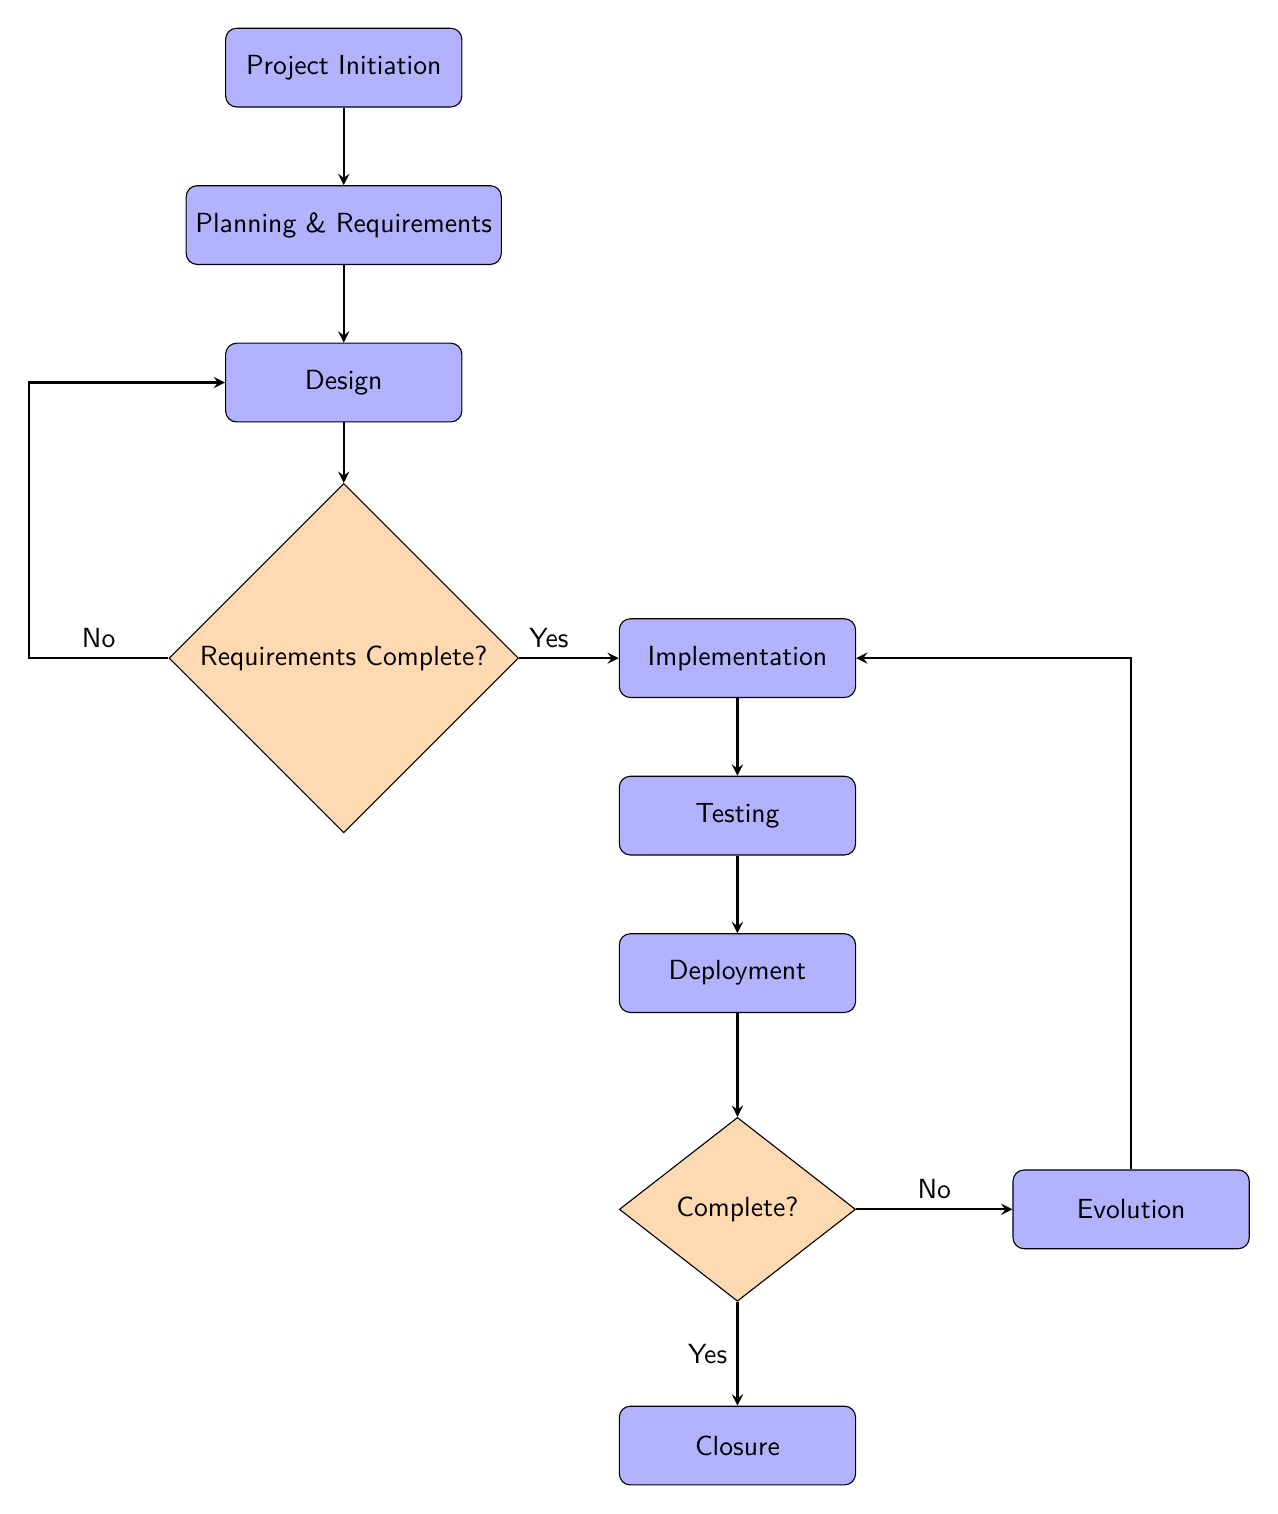
\begin{tikzpicture}[node distance=2cm]

\tikzstyle{process} = [rectangle, rounded corners, minimum width=3cm, minimum height=1cm, text centered, draw=black, fill=blue!30]
\tikzstyle{decision} = [diamond, minimum width=3cm, minimum height=1cm, text centered, draw=black, fill=orange!30]
\tikzstyle{arrow} = [thick,->,>=stealth]

\node (start) [process] {Project Initiation};
\node (planning) [process, below of=start] {Planning \& Requirements};
\node (design) [process, below of=planning] {Design};
\node (decision1) [decision, below of=design, yshift=-1.5cm] {Requirements Complete?};
\node (implement) [process, right of=decision1, xshift=3cm] {Implementation};
\node (test) [process, below of=implement] {Testing};
\node (deploy) [process, below of=test] {Deployment};
\node (decision2) [decision, below of=deploy, yshift=-1.0cm] {Complete?};
\node (evolution) [process, right of=decision2, xshift=3cm] {Evolution};
\node (end) [process, below of=decision2, yshift=-1cm] {Closure};

\draw [arrow] (start) -- (planning);
\draw [arrow] (planning) -- (design);
\draw [arrow] (design) -- (decision1);
\draw [arrow] (decision1) -- node[pos=0.3, above] {Yes} (implement);
\draw [arrow] (decision1) -- node[anchor=south] {No} ++(-4cm,0) |- (design);
\draw [arrow] (implement) -- (test);
\draw [arrow] (test) -- (deploy);
\draw [arrow] (deploy) -- (decision2);
\draw [arrow] (decision2) -- node[anchor=east] {Yes} (end);
\draw [arrow] (decision2) -- node[anchor=south] {No} (evolution);
\draw [arrow] (evolution) |- (implement);

\end{tikzpicture}
\caption{SDLC Flowchart: Development process overview}
\label{fig:sdlc_flowchart}
\end{figure}

\pagebreak

\section{Project Timeline and Gantt Chart}
\label{sec:gantt}

The project was executed in 4 phases over 11 weeks with assigned leads:

\begin{itemize}
  \item \textbf{Phase 1 (Planning):} 2 weeks
  \item \textbf{Phase 2 (Development):} 6 weeks
  \item \textbf{Phase 3 (Security):} 2 weeks
  \item \textbf{Phase 4 (Deployment):} 1 week
\end{itemize}

\begin{figure}[H]
\centering
\includegraphics[width=0.95\textwidth]{gantt.png}
\caption{Project Gantt Chart: Timeline and resource allocation}
\label{fig:gantt_chart}
\end{figure}

\section{Risk Management}
\label{sec:risk_management}

\subsection{Risk Matrix}
\label{sec:risk_matrix}

The risk matrix below provides a framework for assessing the level of risk for potential project setbacks based on the product of likelihood and impact. This enabled the team to prioritize solutions for higher risk issues.
\begin{table}[H]
\centering
\includegraphics[width=0.85\textwidth]{figures/risk_matrix.png}
\caption{Risk Matrix}
\label{fig:risk_matrix}
\end{table}

\subsection{Risk Register}
\label{sec:risk_Register}

\begin{table}[H]
\centering
\includegraphics[width=0.85\textwidth]{figures/risk_register.png}
\caption{Risk Assessment Matrix}
\label{fig:risk_register}
\end{table}

% ============================================================================
\chapter{Requirement Analysis}
\label{ch:requirements}

Requirements specify what the system must do and how it achieves those goals. Detailed implementation, UI/UX, and architecture are described in the Design chapter.

\section{Functional Requirements}
\label{sec:func_req}

Functional requirements define the core behaviors and services the user can interact with.
\begin{itemize}
  \item FR-1: Identity Management: The system must provide a secure registration and local authentication loop, supplemented by remote OAuth 2.0 integration.
  \item FR-2: Social Connectivity: Users must be able to manage unique profiles and establish bidirectional "friend" relationships.
  \item FR-3: Competitive Gameplay: The platform must support a server-authoritative Pong engine providing three distinct modes: Campaign (AI), Arcade (upto 2v2), and Tournament (Multiplayer).
  \item FR-4: Tournament Integrity: The system must automate bracket progression for up to 8 players and commit final rankings to an immutable ledger.
\end{itemize}

\section{Technical Constraints}
\label{sec:tech_req}

Technical constraints define the mandatory architecture and stack limitations imposed on the solution.
\begin{itemize}
  \item TC-1: Microservices Topology: The backend must be decomposed into independent, containerized services orchestrated via Docker.
  \item TC-2: Networking \& Security: All external traffic must be routed through a centralized Nginx gateway enforcing HTTPS and a Web Application Firewall (WAF).
  \item TC-3: Data Sovereignty: Each microservice must maintain its own isolated SQLite database, ensuring no cross-service database coupling.
  \item TC-4: Performance Baseline: The game loop must maintain a server-side execution rate of 60 FPS with state synchronization sent at approx. 16ms intervals.
\end{itemize}

\section{Non-Functional Requirements}
\label{sec:non_func_req}

Non-functional requirements specify the quality attributes and environmental constraints of the system.
\begin{itemize}
  \item NFR-1: Security (Defense-in-Depth): The system must implement six protective layers, including bcrypt password hashing (cost factor 10+), parameterized SQL to prevent injection, and centralized secrets management via HashiCorp Vault.
  \item NFR-2: Availability \& Resilience: Services must implement health checks and automatic restart policies to maintain a 99.9\% uptime target during operation.
  \item NFR-3: Frontend Responsiveness: The Single-Page Application (SPA) must provide a high-fidelity 3D experience using Babylon.js while maintaining a graceful 2D fallback for lower-end hardware.
  \item NFR-4: Scalability: The architecture must support horizontal scaling and handle at least 100+ concurrent WebSocket connections per instance without latency degradation.
\end{itemize}

% ============================================================================
\chapter{Design}
\label{ch:design}
\vspace{-25pt}

\section{System Architecture}
\label{sec:architecture}

The system employs a microservices architecture and the complete deployment consists of 9 Docker containers orchestrated via Docker Compose:

\begin{figure}[H]
\centering
\vspace{-8pt}
\includegraphics[width=0.85\textwidth]{architecture_diagram.png}
\caption{System Architecture with Microservices, API Gateway, and Persistent Storage}
\label{fig:architecture_diagram}
\end{figure}

\section{Data Model}
\label{sec:data_model}

Each microservice manages its own SQLite database:

\subsection{Auth Service Database (auth.db)}
\begin{itemize}
  \item \texttt{users}: id, username, email, password\_hash, oauth\_provider, created\_at, last\_login
\end{itemize}

\subsection{User Service Database (users.db)}
\begin{itemize}
  \item \texttt{user\_profiles}: id, user\_id, display\_name, avatar\_url, is\_custom\_avatar, bio, country, campaign\_level, games\_played, games\_won, win\_streak, tournaments\_won, friends\_count, xp, level, created\_at, updated\_at
  \item \texttt{friends}: user\_id, friend\_id, created\_at
\end{itemize}

\subsection{Game Service Database (games.db)}
\begin{itemize}
  \item \texttt{games}: id, player1\_id, player2\_id, player1\_score, player2\_score, status, started\_at, finished\_at, winner\_id, game\_mode, team1\_players, team2\_players, tournament\_id, tournament\_match\_id
  \item \texttt{game\_events}: id, game\_id, event\_type, event\_data, timestamp
\end{itemize}


\subsection{Tournament Service Database (tournaments.db)}
\begin{itemize}
  \item \texttt{tournaments}: id, name, current\_participants, status, created\_by, created\_at, started\_at, finished\_at, winner\_id
  \item \texttt{tournament\_matches}: id, tournament\_id, round, match\_number, player1\_id, player2\_id, winner\_id, player1\_score, player2\_score, status, played\_at
  \item \texttt{tournament\_participants}: id, tournament\_id, user\_id, alias, avatar\_url, joined\_at, eliminated\_at, final\_rank
\end{itemize}

\newpage

\section{Security Design}
\label{sec:security_design}

The system implements a comprehensive, defense-in-depth security architecture following industry best practices and OWASP guidelines. The security model encompasses six distinct layers, each providing specific protections against various attack vectors.

\begin{figure}[H]
\centering
\includegraphics[width=0.95\textwidth]{security_layers.png}
\caption{Defense-in-Depth Security Architecture with Six Protective Layers}
\label{fig:security_layers}
\end{figure}

\subsection{Layer 1: Network Security}

\subsubsection{HTTPS and TLS Implementation}
All communication channels are secured with HTTPS using TLS 1.2+ protocols.
The system implements:
\begin{itemize}
  \item \textbf{TLS 1.2/1.3 Enforcement:} Nginx configured to reject TLS 1.1 and lower
  \item \textbf{HSTS Headers:} Strict-Transport-Security with max-age=31536000
  \item \textbf{Certificate Validation:} Mutual TLS authentication between services
\end{itemize}

\subsubsection{Web Application Firewall (WAF)}
ModSecurity v3 engine is integrated as an inline module within the Nginx reverse proxy, utilizing the OWASP Core Rule Set (CRS) for real-time traffic inspection to block common attacks.

\subsubsection{Rate Limiting and DDoS Protection}
Nginx implements distributed rate limiting:
\begin{itemize}
  \item \textbf{Request Rate Limiting:} 100 requests per minute per IP
  \item \textbf{Burst Protection:} Queue-based rate limiting with burst allowance
  \item \textbf{Distributed State:} Redis-backed rate limiting across multiple instances
\end{itemize}

\subsection{Layer 2: Transport Security}

\subsubsection{Mutual TLS (mTLS) Between Services}
All inter-service communication uses mutual TLS authentication.

\subsubsection{Session Security}
Redis-backed session storage with TLS encryption:
\begin{itemize}
  \item \textbf{Secure Session Storage:} Sessions stored in Redis with TLS encryption
  \item \textbf{Session Encryption:} All session data encrypted in transit and at rest
  \item \textbf{Session Timeout:} Automatic session expiration and cleanup
\end{itemize}

\subsection{Layer 3: Application Security}

\subsubsection{Input Validation and Sanitization}
Comprehensive input validation using manual checks and sanitization.

\subsubsection{SQL Injection Prevention}
All SQL queries use parameterized statements with $`?`$ placeholders.

\subsubsection{Cross-Site Scripting (XSS) Protection}
Multiple layers of XSS prevention:
\begin{itemize}
  \item \textbf{Content Security Policy (CSP):} Strict CSP headers enforced
  \item \textbf{X-XSS-Protection:} Browser-based XSS filtering enabled
  \item \textbf{Input Sanitization:} All user inputs sanitized before rendering
\end{itemize}

\subsubsection{Cross-Site Request Forgery (CSRF) Protection}
CSRF protection via SameSite cookie attributes and origin validation.

\subsection{Layer 4: Authentication \& Authorization}

\subsubsection{Password Security}
Industry-standard password hashing and validation.

\subsubsection{Multi-Factor Authentication (MFA)}
OAuth 2.0 integration with Google OAuth for enhanced authentication.

\subsection{Layer 5: Data Protection}

\subsubsection{Secrets Management with HashiCorp Vault}
Centralized secrets management for all sensitive data. Key secrets managed in Vault:
\begin{itemize}
  \item \textbf{API Keys:} OAuth provider secrets and external service keys
  \item \textbf{Session Secrets:} Cryptographically secure session signing keys
  \item \textbf{TLS Certificates:} Automated certificate lifecycle management
\end{itemize}

\subsubsection{Database Security}
SQLite databases with additional security measures:
\begin{itemize}
  \item \textbf{Prepared Statements:} All queries use parameterized execution
  \item \textbf{Connection Pooling:} Efficient resource management
  \item \textbf{Access Control:} Database files with restricted permissions
\end{itemize}

\subsection{Layer 6: Monitoring \& Logging}

\subsubsection{Security Event Logging}
Comprehensive logging of security-relevant events.

\subsubsection{Health Monitoring}
Automated health checks for all security components:
\begin{itemize}
  \item \textbf{Certificate Expiry Monitoring:} Automatic renewal alerts
  \item \textbf{Vault Connectivity:} Health checks for secrets management
  \item \textbf{WAF Status:} ModSecurity rule effectiveness monitoring
\end{itemize}

\subsection{Layer 7: Incident Response}

\subsubsection{Security Headers Implementation}
Comprehensive security headers configuration implemented within the \texttt{nginx.conf} file.

\subsubsection{Container Security}
Docker security best practices implementation:
\begin{itemize}
  \item \textbf{Non-root Users:} All containers run as non-privileged users
  \item \textbf{Minimal Images:} Alpine Linux base images for reduced attack surface
  \item \textbf{Secret Management:} Environment variables and Vault retrievals for sensitive configuration
  \item \textbf{Resource Limits:} Memory and CPU limits to prevent resource exhaustion
\end{itemize}

\pagebreak

\subsection{Security Testing and Validation}

The security implementation is validated through comprehensive testing:

\subsubsection{WAF Effectiveness Testing}
Tests verify ModSecurity rule effectiveness:
\begin{itemize}
  \item \textbf{SQL Injection Attempts:} Parameterized query validation
  \item \textbf{XSS Payload Testing:} Input sanitization verification
  \item \textbf{Path Traversal:} File system access control validation
\end{itemize}

\subsubsection{Vault Integration Testing}
Secrets management functionality validation:
\begin{itemize}
  \item \textbf{Secret Retrieval:} Automated secret access testing
  \item \textbf{Certificate Management:} PKI certificate lifecycle testing
\end{itemize}

\subsubsection{HTTPS/TLS Testing}
Transport security validation:
\begin{itemize}
  \item \textbf{Certificate Validation:} SSL/TLS handshake verification
  \item \textbf{Cipher Suite Testing:} Supported cipher suite validation
  \item \textbf{HSTS Compliance:} Security header presence verification
\end{itemize}

\subsection{Security Compliance}

The implementation achieves compliance with multiple security standards:

\subsubsection{OWASP Top 10 Coverage}
\begin{itemize}
  \item \textbf{A01:2021 - Broken Access Control:} Session validation
  \item \textbf{A02:2021 - Cryptographic Failures:} TLS 1.2+ and bcrypt hashing
  \item \textbf{A03:2021 - Injection:} Parameterized queries and input validation
  \item \textbf{A04:2021 - Insecure Design:} Defense-in-depth architecture
  \item \textbf{A05:2021 - Security Misconfiguration:} Automated configuration validation
\end{itemize}

\subsubsection{Industry Best Practices}
\begin{itemize}
  \item \textbf{Zero Trust Architecture:} Every request authenticated and authorized
  \item \textbf{Least Privilege:} Minimal permissions for all components
  \item \textbf{Fail-Safe Defaults:} Secure defaults with explicit allow rules
  \item \textbf{Defense in Depth:} Multiple security layers for redundancy
\end{itemize}

\section{Blockchain Integration}
\label{sec:blockchain}

The ft\_transcendence platform uses blockchain technology to provide immutable tournament result recording, improving transparency and reducing the risk of result manipulation. The implementation runs on a local Hardhat network inside Docker and is suitable for development, testing, and staging demonstrations.

\subsection{Blockchain Architecture}

The blockchain implementation consists of four coordinated components:

\begin{enumerate}
  \item \textbf{Hardhat Local Network:} Dockerized Ethereum-compatible network used for local execution.
  \item \textbf{Solidity Smart Contract:} On-chain tournament ranking storage with owner-restricted write access.
  \item \textbf{Deployment Step:} Automated contract deployment that persists the deployed address for service startup.
  \item \textbf{Blockchain Service:} Internal API that receives rankings and submits transactions to the smart contract.
\end{enumerate}

\begin{figure}[H]
\centering
\includegraphics[width=0.55\textwidth]{12_blockchain_record.png}
\caption{Blockchain Record: Tournament Result Verification on Immutable Ledger}
\label{fig:blockchain_record}
\end{figure}

\subsection{Smart Contract Implementation}

The smart contract stores tournament rankings by tournament identifier and player identifier. Writes are restricted to the contract owner, and each recorded rank emits an event for traceability.

\subsubsection{Contract Features}
\begin{itemize}
  \item \textbf{Immutability:} Tournament results cannot be altered once recorded
  \item \textbf{Access Control:} Only the authorized owner account can record results
  \item \textbf{Batch Submission:} Multiple player ranks can be recorded in a single transaction
  \item \textbf{Event Logging:} Transparent event emission for result verification
\end{itemize}

\subsection{Hardhat Development Environment}

The project uses Hardhat as its local blockchain runtime for development and validation. The runtime is configured for an internal Docker network and deterministic local chain ID behavior.

\subsubsection{Deployment Automation}
Contract deployment is automated during container startup. The deployed contract address is persisted and consumed by the blockchain service, preventing manual copy/paste steps and reducing integration drift.

\subsection{Blockchain Service Architecture}

The blockchain service exposes an internal API for tournament result recording.

\subsubsection{Service Components}
\begin{itemize}
  \item \textbf{Network Connectivity:} Connection to the local Hardhat node over the internal Docker network
  \item \textbf{Key Management:} Runtime retrieval of signing key material from HashiCorp Vault
  \item \textbf{Contract Binding:} Initialization from deployed address and compiled contract artifact
  \item \textbf{Transaction Confirmation:} Return of mined transaction hash for traceability
\end{itemize}

\subsubsection{Service Behavior}
At startup, the service validates required blockchain artifacts and deployment metadata, then initializes contract access. During requests, payloads are validated, rankings are submitted in batch, and transaction hashes are returned to upstream services.

\subsection{Tournament Integration}

Tournament results are automatically recorded to blockchain upon completion:

\subsubsection{Integration Flow}
\begin{enumerate}
  \item Tournament matches complete and final rankings determined
  \item Tournament service calls blockchain service with player rankings
  \item Blockchain service submits transaction to smart contract
  \item Transaction hash returned and stored in tournament database
  \item Results become immutable and verifiable on blockchain
\end{enumerate}

\subsection{Blockchain Security Measures}

\subsubsection{Private Key Management}
\begin{itemize}
  \item \textbf{Vault Storage:} Private keys stored securely in HashiCorp Vault
  \item \textbf{Runtime Retrieval:} Keys loaded at service startup, not persisted
  \item \textbf{Access Control:} Microservice authentication via shared secrets
  \item \textbf{Audit Logging:} All blockchain operations logged with transaction details
\end{itemize}

\subsubsection{Transaction Security}
\begin{itemize}
  \item \textbf{Authorization Checks:} Requests are accepted only from authenticated sessions or trusted internal callers
  \item \textbf{Transaction Confirmation:} Responses include mined transaction hashes for verification
  \item \textbf{Input Validation:} Tournament identifier and ranking payloads are validated before submission
  \item \textbf{Failure Signaling:} Failed submissions return explicit error responses for upstream handling
\end{itemize}

\subsection{Blockchain Testing and Validation}

Validation activities cover contract deployment, transaction submission, and end-to-end integration from tournament completion to recorded on-chain result.

\subsubsection{Contract Testing}
\begin{itemize}
  \item \textbf{Compilation and Deployment Checks:} Validation that contract artifacts and deployment metadata are generated
  \item \textbf{Functional Validation:} Verification of rank recording and retrieval behavior
  \item \textbf{Integration Validation:} End-to-end checks from tournament flow to on-chain transaction
  \item \textbf{Security Review:} Manual review of access control and input assumptions
\end{itemize}

\subsubsection{Service Testing}
Service tests validate API authorization, payload validation, and transaction result handling.

\subsection{Blockchain Performance Optimization}

\subsubsection{Gas Optimization}
\begin{itemize}
  \item \textbf{Batch Operations:} Multiple rankings recorded in single transaction
  \item \textbf{Efficient Storage:} Mapping-based storage for straightforward lookup
  \item \textbf{Minimal Computation:} Simple ranking storage without complex logic
\end{itemize}

\subsubsection{Network Efficiency}
\begin{itemize}
  \item \textbf{Local Network:} Hardhat provides fast local blockchain operations for development and testing
  \item \textbf{Async Processing:} Non-blocking blockchain operations in tournament flow
  \item \textbf{Preloaded Metadata:} Contract address and artifact data loaded at service startup
\end{itemize}

\subsection{Blockchain Monitoring and Observability}

\subsubsection{Transaction Monitoring}
\begin{itemize}
  \item \textbf{Transaction Hashes:} All blockchain operations tracked with unique identifiers
  \item \textbf{Event Logging:} Smart contract events logged for audit trails
  \item \textbf{Performance Metrics:} Gas usage and transaction time monitoring
  \item \textbf{Error Tracking:} Failed transactions logged with detailed error information
\end{itemize}

\subsubsection{Health Checks}
Automated health monitoring for blockchain components:
\begin{itemize}
  \item \textbf{Network Connectivity:} Hardhat node availability monitoring
  \item \textbf{Contract Accessibility:} Smart contract address validation
  \item \textbf{Service Health:} Blockchain service API responsiveness
\end{itemize}

\subsection{Blockchain Deployment and Operations}

\subsubsection{Docker Integration}
The blockchain node, deployment step, and blockchain service are containerized and orchestrated together. Service startup is dependency-aware: the node becomes healthy first, contract deployment completes, then the API service starts with mounted artifacts and deployment metadata.

\subsubsection{Production Considerations}
\begin{itemize}
  \item \textbf{Current Scope:} Local-chain deployment focused on development, testing, and subject validation
  \item \textbf{Public-Network Migration:} Requires external RPC providers, secure key lifecycle controls, and chain-specific gas policies
  \item \textbf{Operational Hardening:} Requires enhanced observability, alerting, and incident procedures for sustained production use
  \item \textbf{Resilience Planning:} Requires deployment/versioning strategy for contract upgrades and rollback-safe service releases
\end{itemize}

This blockchain integration provides tournament result immutability and transparency, ensuring competitive outcomes can be independently verified. The implementation demonstrates practical blockchain integration for a microservice system in development and staging contexts, with a clear path to additional production hardening.

\section{Microservices Architecture}
\label{sec:microservices}

The ft\_transcendence platform implements a comprehensive microservices architecture designed for scalability, maintainability, and fault isolation. The system consists of 8 containerized services orchestrated through Docker Compose using a \texttt{docker-compose.yml} file, with each service handling specific business domains and communicating through well-defined APIs.

\subsection{Deployment Topology}

The microservices architecture follows domain-driven design principles with clear separation of concerns:

\begin{enumerate}
  \item \textbf{Vault Service:} HashiCorp Vault for secrets management and certificate management
  \item \textbf{Redis Service:} In-memory data store for session management and caching
  \item \textbf{Auth Service:} User authentication and authorization with session tokens
  \item \textbf{User Service:} User profile management and social features
  \item \textbf{Game Service:} Real-time game logic and WebSocket communication
  \item \textbf{Tournament Service:} Tournament management and bracket generation
  \item \textbf{Blockchain Service:} Smart contract interaction and transaction management
  \item \textbf{Frontend Service:} React-based SPA with 3D Babylon.js rendering
\end{enumerate}

\begin{figure}[H]
\centering
\includegraphics[width=0.8\textwidth]{deployment_topology.png}
\caption{Deployment Topology: Service Dependencies and Communication Flow}
\label{fig:microservices_architecture}
\end{figure}

\subsection{Service Communication Patterns}

Services communicate through multiple protocols optimized for different use cases:

\begin{itemize}
  \item \textbf{HTTP/HTTPS APIs:} RESTful communication between services using Fastify framework
  \item \textbf{WebSocket Connections:} Real-time game state synchronization
  \item \textbf{Database Sharing:} SQLite databases with service-specific schemas
  \item \textbf{Shared Volumes:} Persistent data storage with bind mounts
  \item \textbf{Environment Variables:} Configuration management through .env files
\end{itemize}

\subsection{Service Health Monitoring}

Each service implements comprehensive health checks with automatic restart policies:

\begin{itemize}
  \item \textbf{Health Endpoints:} HTTP health checks on service-specific ports
  \item \textbf{Dependency Validation:} Services wait for dependencies before starting
  \item \textbf{Resource Limits:} Memory and CPU constraints per service (256MB limit)
  \item \textbf{Startup Probes:} Extended startup periods for complex services
  \item \textbf{Retry Logic:} Automatic restart on failure with exponential backoff
\end{itemize}

\subsection{Database Architecture}

The platform uses SQLite databases with service-specific schemas and cross-service data sharing:

\begin{itemize}
  \item \textbf{Auth Database:} User credentials and session tokens
  \item \textbf{User Database:} Profile and social data
  \item \textbf{Game Database:} Match history and game statistics
  \item \textbf{Tournament Database:} Tournament brackets and results
  \item \textbf{Vault Database:} Encrypted secrets and certificates
\end{itemize}

\subsection{Production Deployment Considerations}

The microservices architecture supports production deployment with:

\begin{itemize}
  \item \textbf{Load Balancing:} Nginx reverse proxy for service distribution
  \item \textbf{Service Discovery:} Internal DNS resolution within Docker network
  \item \textbf{Configuration Management:} Environment-based configuration
  \item \textbf{Logging Aggregation:} Centralized logging through Docker Compose
  \item \textbf{Monitoring Integration:} Health check endpoints for external monitoring
\end{itemize}

This microservices architecture provides the foundation for a scalable, maintainable platform with clear service boundaries, comprehensive testing, and production-ready deployment capabilities.

\pagebreak

\section{3D Frontend Implementation}
\label{sec:3d_frontend}

The ft\_transcendence platform features an innovative 3D user interface built with Babylon.js, providing an immersive gaming experience that transcends traditional 2D web applications. The 3D frontend combines modern web technologies with advanced 3D rendering techniques.

\subsection{Immersive Office Environment}
The application features a unique "Immersive Office" concept where the user interacts with the application through a virtual computer monitor situated within a 3D rendered 90s-style office cubicle. This design choice transforms the standard web interface into a diegetic element of the game world, enhancing immersion.

The 3D environment serves as more than just a background; it is the primary container for the application. When the user navigates the application, they are effectively looking at the screen of the virtual monitor.

\begin{figure}[H]
\centering
\includegraphics[width=0.8\textwidth]{figures/3D_monitor_main_menu.png}
\caption{Immersive Office: Main Menu displayed on the Virtual Monitor}
\label{fig:3d_monitor_main_menu}
\end{figure}

\subsection{Story and Lore Integration}
Upon the first launch, the user is presented with a narrative sequence that establishes the setting. The camera acts as the user's viewpoint, capable of panning dynamically between different points of interest, such as the monitor (for gameplay and UI) and "Lore" items (like newspapers) scattered around the desk.

This seamless transition is managed by the \texttt{BabylonWrapper}, which interpolates camera positions to create smooth, cinematic movements between these interaction points, making the UI feel like an integrated part of the story.

\begin{figure}[H]
\centering
\includegraphics[width=0.6\textwidth]{figures/3D_newspaper_view.png}
\caption{Story Integration: Interactive Newspaper providing Narrative Context}
\label{fig:3d_newspaper_view}
\end{figure}

\subsection{Babylon.js Integration Architecture}

The 3D frontend implementation uses a singleton pattern with conditional initialization to manage the scene, camera, and post-processing effects. The helper methods \texttt{panToLore()} and \texttt{panToMonitor()} handle the cinematic transitions.


\subsection{3D Game Rendering and Environmental Effects}

The 3D Pong game is not an isolated overlay but plays out physically within the 3D scene. The game board is positioned effectively "inside" the virtual monitor.

\subsubsection{Environmental Lighting Interaction}
A key feature of the 3D mode is the interplay between game elements and the environment. The ball and paddles are equipped with dynamic light sources. As the ball moves across the field, it casts real-time light onto the surrounding office desk and objects, creating a grounded and realistic effect. The virtual monitors also emit a glow that reflects off the desk surface.

\begin{figure}[H]
\centering
\includegraphics[width=0.8\textwidth]{figures/3D_TV_arcade_game.png}
\caption{3D Arcade Mode: Rendering "Inside" the Virtual TV Screen}
\label{fig:3d_tv_arcade_game}
\end{figure}

\subsection{Real-time 3D Synchronization}

The 3D renderer synchronizes with WebSocket game state updates:

\begin{itemize}
  \item \textbf{Coordinate Mapping:} 2D game coordinates mapped to 3D world space
  \item \textbf{Smooth Interpolation:} Ball and paddle movement with easing functions
  \item \textbf{Visual Effects:} Dynamic lighting, particle trails, and glow effects
\end{itemize}

\subsection{HTML Mesh Integration}

To achieve the "game within a monitor" effect for standard UI pages, the system employs Babylon.js's \texttt{HtmlMesh}. This allows the existing DOM-based interface (React/Vanilla JS) to be projected onto a 3D plane within the scene, maintaining full interactivity (clicking, scrolling) while undergoing 3D perspective transformations.


\subsection{Post-Processing Effects}

Advanced visual effects enhance the retro gaming aesthetic:

\begin{itemize}
  \item \textbf{Ambient Occlusion:} SSAO for realistic shadow rendering
  \item \textbf{Depth of Field:} Lens effects for cinematic camera work
  \item \textbf{Fog Effects:} Atmospheric depth cueing
  \item \textbf{Glow Layers:} Neon lighting effects for retro aesthetic
\end{itemize}

\subsection{Performance Optimizations}

The 3D implementation includes comprehensive performance optimizations:

\begin{itemize}
  \item \textbf{Conditional Rendering:} 3D mode only enabled when WebGL is available
  \item \textbf{Resource Management:} Proper cleanup and disposal of 3D resources
  \item \textbf{Memory Limits:} Texture compression and efficient mesh usage
  \item \textbf{Fallback Support:} Graceful degradation to 2D rendering
\end{itemize}

This 3D frontend implementation provides an innovative, immersive gaming experience while maintaining performance and accessibility standards.

\pagebreak

\section{Wireframes and User Interface Design}
\label{sec:wireframes_design}

Wireframes provide visual representations of application screens, illustrating layout, functionality, and user navigation flow. The design follows human-computer interaction principles with intuitive navigation and clear visual hierarchy.

\subsection{Authentication Flow Wireframes}

\subsubsection{Login Interface}
\begin{figure}[H]
\centering
\includegraphics[width=0.9\textwidth]{figures/flow_login.png}
\caption{Authentication User Flow: Diagram illustrating the user journey through login and registration screens}
\label{fig:auth_flow_diagram}
\end{figure}

\begin{figure}[H]
\centering
\includegraphics[width=0.8\textwidth]{figures/wireframe_login.png}
\caption{Login Interface Wireframe: Email/password authentication layout}
\label{fig:login_wireframe}
\end{figure}

Key elements:
\begin{itemize}
  \item "Register" tab for new user registration
  \item Email and password input fields with validation
  \item "Login" button
  \item Google OAuth integration button
  \item Error message display area
\end{itemize}

\subsubsection{Registration Interface}
\begin{figure}[H]
\centering
\includegraphics[width=0.8\textwidth]{figures/wireframe_register.png}
\caption{Registration Interface Wireframe: New user account creation form layout}
\label{fig:registration_wireframe}
\end{figure}

Key elements:
\begin{itemize}
  \item "Login" tab for existing user authentication
  \item Username, email, and password fields
  \item "Register" button
  \item Error message display area
\end{itemize}

\subsection{Main Navigation and Menu Wireframes}

\subsubsection{Main Menu Interface}
\begin{figure}[htbp]
\centering
\includegraphics[width=0.8\textwidth]{figures/wireframe_main-menu.png}
\caption{Main Menu Wireframe: Navigation hub with game modes and profile access}
\label{fig:main_menu_wireframe}
\end{figure}

Key elements:
\begin{itemize}
  \item Game mode buttons: Campaign, Arcade, Tournament
  \item User profile section with avatar and stats
  \item Settings and logout options
\end{itemize}

\subsection{Game Interface Wireframes}

\subsubsection{Game Mode Selection}
\begin{figure}[htbp]
\centering
\includegraphics[width=0.7\textwidth]{figures/4_playemode_game_settings.png}
\caption{Game Mode Selection: Difficulty and settings configuration}
\label{fig:game_settings_wireframe}
\end{figure}

Key elements:
\begin{itemize}
  \item Difficulty level selector (Easy, Medium, Hard)
  \item Ball speed adjustment slider
  \item Paddle size configuration
  \item AI opponent toggle (for campaign mode)
  \item "Start Game" button
\end{itemize}

\subsubsection{Gameplay Interface}
\begin{figure}[htbp]
\centering
\includegraphics[width=0.8\textwidth]{figures/wireframe_game.png}
\caption{Gameplay Interface Wireframe: Pong match layout with HUD elements}
\label{fig:gameplay_wireframe}
\end{figure}

Key elements:
\begin{itemize}
  \item Game canvas/board area
  \item Real-time score display (Player 1 vs Player 2)
  \item Game status text indicator
  \item 3D/2D rendering toggle feedback
\end{itemize}

\subsubsection{Multiplayer Arcade Mode}
\begin{figure}[htbp]
\centering
\includegraphics[width=0.8\textwidth]{figures/multiplayer_arcade.png}
\caption{Multiplayer Arcade: Real-time competitive gameplay}
\label{fig:multiplayer_wireframe}
\end{figure}

Key elements:
\begin{itemize}
  \item Player identification (avatars/names)
  \item Real-time input synchronization
  \item Disconnect/reconnect handling
\end{itemize}

\subsection{Tournament Interface Wireframes}

\subsubsection{Tournament Bracket View}
\begin{figure}[htbp]
\centering
\includegraphics[width=0.8\textwidth]{figures/tournament_bracket_matches.png}
\caption{Tournament Bracket: Match scheduling and progression visualization}
\label{fig:tournament_bracket_wireframe}
\end{figure}

Key elements:
\begin{itemize}
  \item Interactive bracket visualization
  \item Current match highlighting
  \item Participant status indicators
  \item Blockchain recording status message
  \item Player elimination tracking
\end{itemize}

\subsubsection{Tournament Mode Selection}
\begin{figure}[htbp]
\centering
\includegraphics[width=0.8\textwidth]{figures/gamemode_tournament.png}
\caption{Tournament Mode Selection: Tournament creation and joining interface}
\label{fig:tournament_mode_wireframe}
\end{figure}

Key elements:
\begin{itemize}
  \item "Create Tournament" button
  \item Available tournaments list
  \item Tournament details (players, prize, status)
  \item Join/registration functionality
  \item Tournament rules display
\end{itemize}

\subsection{User Profile and Social Features}

\subsubsection{Dashboard and Profile}
\begin{figure}[htbp]
\centering
\includegraphics[width=0.8\textwidth]{figures/13_dashboard_profile.png}
\caption{User Dashboard: Profile statistics and achievements}
\label{fig:dashboard_wireframe}
\end{figure}

Key elements:
\begin{itemize}
  \item User avatar and bio
  \item Win/Loss statistics visualization
  \item Match history with expansion details
  \item Friend list and social actions
\end{itemize}

\subsection{3D Environment Integration}

\subsubsection{3D Monitor Interface}
\begin{figure}[htbp]
\centering
\includegraphics[width=0.8\textwidth]{figures/3D_monitor_main_menu.png}
\caption{3D Monitor Interface: Main menu projected on virtual screen}
\label{fig:3d_monitor_wireframe}
\end{figure}

Key elements:
\begin{itemize}
  \item 3D office environment context
  \item Virtual monitor displaying UI
  \item Interactive HTML mesh projection
  \item Environmental lighting effects
  \item Camera controls for 3D navigation
\end{itemize}

\subsubsection{3D Arcade Game Mode}
\begin{figure}[htbp]
\centering
\includegraphics[width=0.8\textwidth]{figures/3D_TV_arcade_game.png}
\caption{3D Arcade Mode: Game rendering within virtual TV screen}
\label{fig:3d_arcade_wireframe}
\end{figure}

Key elements:
\begin{itemize}
  \item Game rendered "inside" virtual monitor
  \item 3D ball and paddle physics
  \item Dynamic lighting from game elements
  \item Environmental interaction effects
  \item Retro aesthetic with modern 3D effects
\end{itemize}

\subsubsection{3D Newspaper/Lore View}
\begin{figure}[htbp]
\centering
\includegraphics[width=0.8\textwidth]{figures/3D_newspaper_view.png}
\caption{3D Newspaper View: Interactive environmental storytelling}
\label{fig:3d_newspaper_wireframe}
\end{figure}

Key elements:
\begin{itemize}
  \item Newspaper mesh in 3D space
  \item Interactive reading experience
  \item Camera transitions and animations
  \item Contextual game information
  \item Immersive narrative elements
\end{itemize}

\subsection{Wireframe Design Principles}

\subsubsection{Responsive Design Considerations}
\begin{itemize}
  \item \textbf{Desktop-First Design:} Optimized for mouse and keyboard interaction
  \item \textbf{High-Performance Layout:} Fixed-width canvas for consistent game rendering
  \item \textbf{Clear Visual Hierarchy:} Prioritized game elements and status indicators
\end{itemize}

\subsubsection{User Experience Guidelines}
\begin{itemize}
  \item \textbf{Intuitive Navigation:} Clear information hierarchy and logical flow
  \item \textbf{Visual Consistency:} Unified color scheme and typography
  \item \textbf{Feedback Systems:} Loading states, success/error messages, and progress indicators
  \item \textbf{Performance Focus:} Optimized for 60 FPS gameplay and responsive interactions
\end{itemize}

\subsubsection{3D Integration Principles}
\begin{itemize}
  \item \textbf{Optional Enhancement:} 3D mode as progressive enhancement over 2D
  \item \textbf{Performance Fallback:} Automatic degradation to 2D rendering when needed
  \item \textbf{Contextual Immersion:} 3D environment enhances rather than complicates gameplay
  \item \textbf{Technical Stability:} WebGL detection and error handling
\end{itemize}

\subsection{Main Menu Interface}
\begin{figure}[H]
\centering
\includegraphics[width=0.55\textwidth]{3_Main_Menu.png}
\caption{Main Menu: Game Mode Selection (Campaign, Arcade, Tournament)}
\label{fig:main_menu}
\end{figure}

The main menu interface was tested for:
\begin{itemize}
  \item Responsive layout across different screen sizes
  \item Navigation to all game modes
  \item Visual consistency with design specifications
  \item Clear navigation structure
\end{itemize}

\subsection{Game Mode Selection}
\begin{figure}[H]
\centering
\includegraphics[width=0.55\textwidth]{game_modes.png}
\caption{Available Game Modes: Campaign, Arcade, Tournament}
\label{fig:game_modes}
\end{figure}

Game mode selection functionality was validated through:
\begin{itemize}
  \item End-to-end user workflow testing
  \item Integration with backend game services
  \item Error handling for invalid selections
  \item Performance under concurrent user load
\end{itemize}

\subsection{Authentication UI Implementation}

The application provides comprehensive authentication screens capturing user credentials securely:

\subsubsection{Login Interface}
\begin{figure}[H]
\centering
\includegraphics[width=0.50\textwidth]{2_login_UI.png}
\caption{Login User Interface: Email/Password Authentication}
\label{fig:login_ui}
\end{figure}

\subsubsection{Registration Interface}
\begin{figure}[H]
\centering
\includegraphics[width=0.50\textwidth]{3_create_new_account_UI.png}
\caption{Account Registration UI: New Account Creation}
\label{fig:register_ui}
\end{figure}

\subsection{Gameplay Interface}
\begin{figure}[H]
\centering
\includegraphics[width=0.55\textwidth]{multiplayer_arcade.png}
\caption{Arcade Multiplayer Mode: Real-Time 1v1 Pong Match with Live Score Display}
\label{fig:arcade_gameplay}
\end{figure}

Real-time gameplay interfaces were tested for:
\begin{itemize}
  \item WebSocket connection stability
  \item Real-time score updates
  \item Input responsiveness (keyboard/mouse)
  \item Visual feedback during gameplay
\end{itemize}

\subsection{Game Settings}
\begin{figure}[H]
\centering
\includegraphics[width=0.55\textwidth]{4_playemode_game_settings.png}
\caption{Game Settings: Difficulty, Ball Speed, Paddle Size Customization}
\label{fig:game_settings}
\end{figure}

Game customization settings were validated for:
\begin{itemize}
  \item Parameter validation and bounds checking
  \item Real-time application of settings
  \item Persistence across game sessions
  \item Impact on game physics and AI behavior
\end{itemize}

\subsection{Campaign Mode}
\begin{figure}[H]
\centering
\includegraphics[width=0.55\textwidth]{Campaign_game_running.png}
\caption{Campaign Mode: Single-Player Progression Against AI Opponent}
\label{fig:campaign_gameplay}
\end{figure}

Campaign progression system was tested for:
\begin{itemize}
  \item Level advancement logic
  \item AI difficulty scaling
  \item Progress persistence and recovery
\end{itemize}

\subsection{Tournament System}
\begin{figure}[H]
\centering
\includegraphics[width=0.55\textwidth]{tournament_bracket_matches.png}
\caption{Tournament Mode: Bracket-Based Competition with Multiple Players}
\label{fig:tournament_mode}
\end{figure}

Tournament functionality was validated through:
\begin{itemize}
  \item Bracket generation algorithms
  \item Multi-player synchronization
  \item Match scheduling and results tracking
  \item Blockchain integration for result verification
\end{itemize}

\subsection{User Profile and Statistics}
\begin{figure}[H]
\centering
\includegraphics[width=0.55\textwidth]{13_dashboard_profile.png}
\caption{User Dashboard: Profile Information, Statistics Overview, Recent Activity}
\label{fig:user_dashboard}
\end{figure}

User profile features were tested for:
\begin{itemize}
  \item Data privacy and compliance
  \item Statistics calculation accuracy
  \item Profile update functionality
  \item Social features integration
\end{itemize}

\pagebreak

% ============================================================================
\section{Flowcharts}
\label{sec:flowcharts}

Flowcharts illustrate the primary user interactions, system processes, and data flow across key components such as the homepage, settings, player profile, chat, and game sections, providing a comprehensive overview of the project's functional workflow.

\subsection{System Workflow Overview}

\begin{figure}[H]
\centering
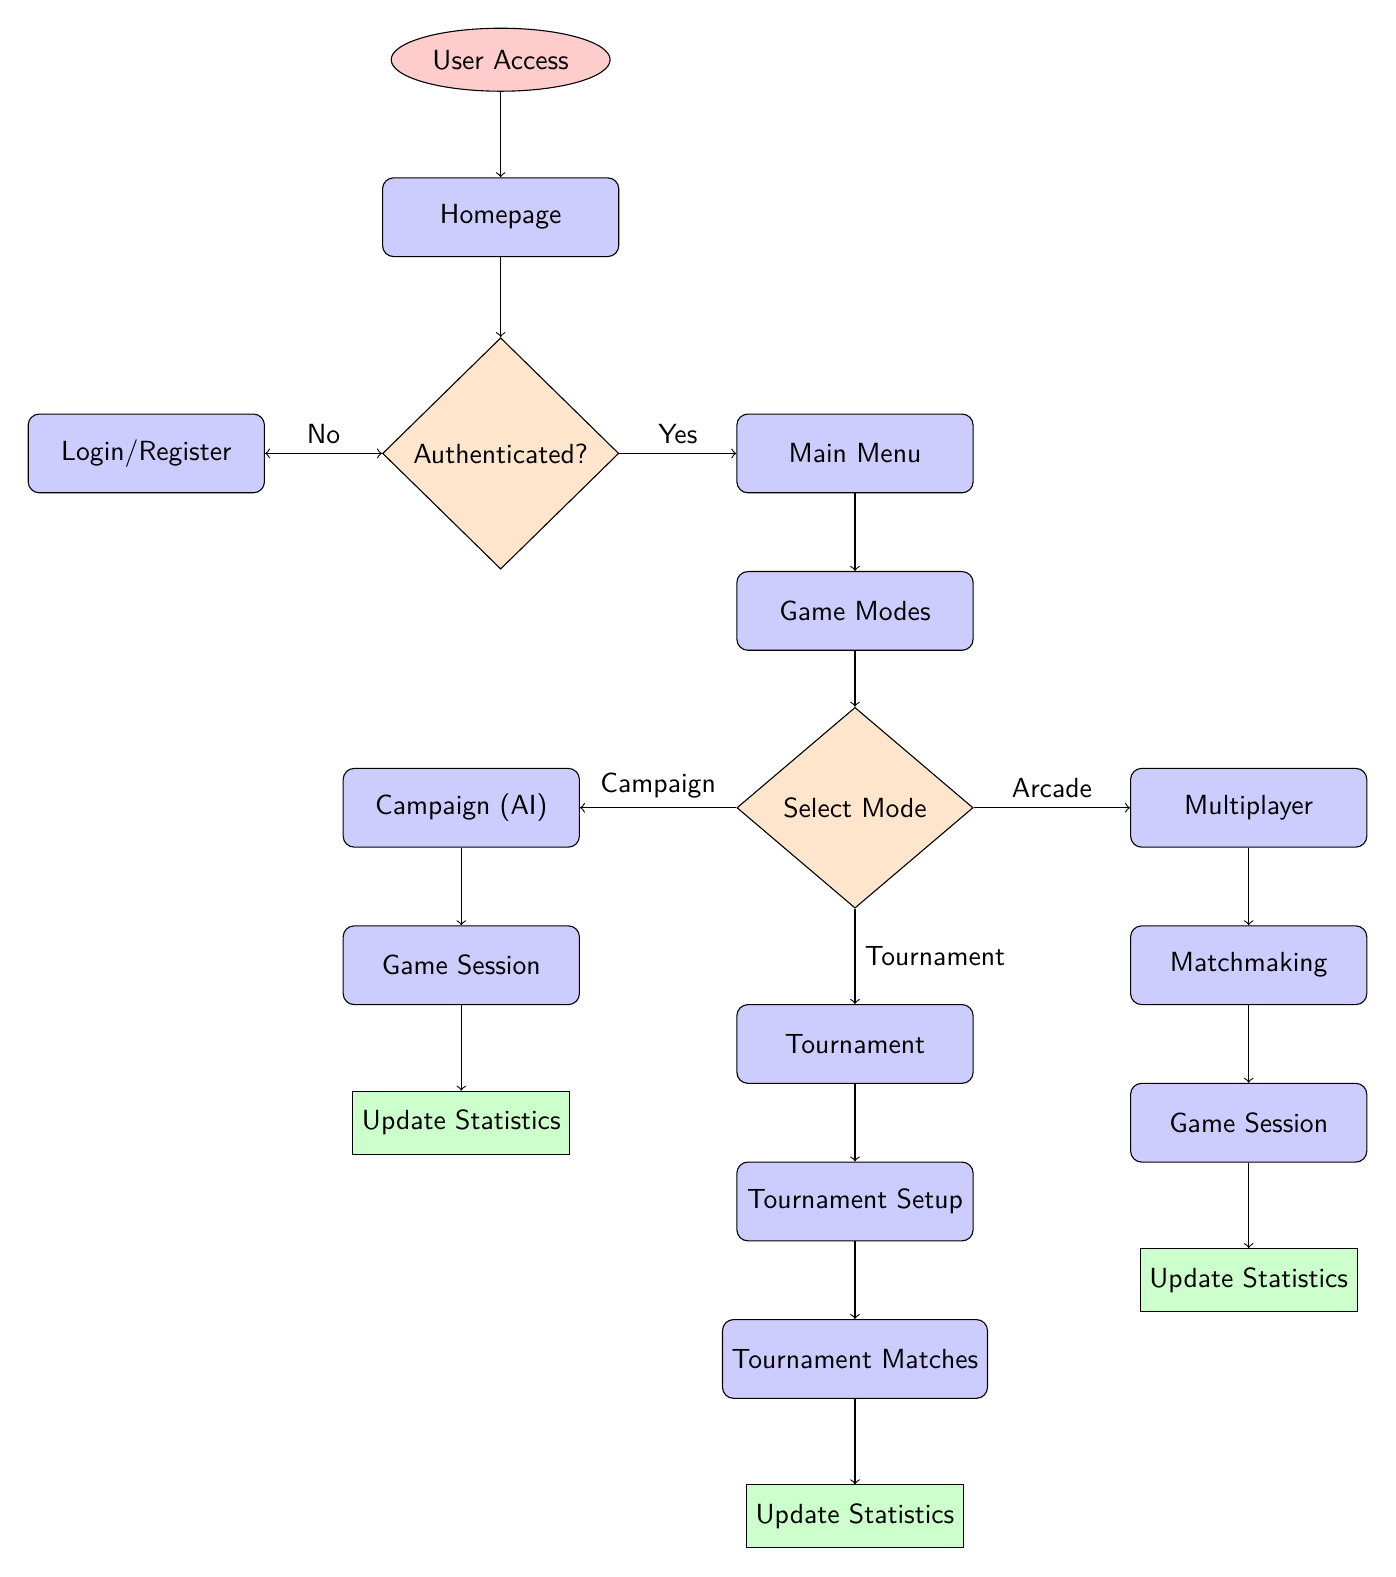
\begin{tikzpicture}[node distance=2cm, auto]
    % Define styles
    \tikzstyle{process} = [rectangle, rounded corners, minimum width=3cm, minimum height=1cm, text centered, draw=black, fill=blue!20]
    \tikzstyle{decision} = [diamond, minimum width=3cm, minimum height=1cm, text centered, draw=black, fill=orange!20]
    \tikzstyle{data} = [rectangle, minimum width=2cm, minimum height=0.8cm, text centered, draw=black, fill=green!20]
    \tikzstyle{startend} = [ellipse, minimum width=2cm, minimum height=0.8cm, text centered, draw=black, fill=red!20]

    % Nodes
    \node[startend] (start) {User Access};
    \node[process, below of=start] (homepage) {Homepage};
    \node[decision, below of=homepage, yshift=-1.0cm] (auth_check) {Authenticated?};
    \node[process, left of=auth_check, xshift=-2.5cm] (login) {Login/Register};
    \node[process, right of=auth_check, xshift=2.5cm] (main_menu) {Main Menu};
    \node[process, below of=main_menu] (game_modes) {Game Modes};
    \node[decision, below of=game_modes, yshift=-0.5cm] (mode_select) {Select Mode};
    \node[process, left of=mode_select, xshift=-3cm] (campaign) {Campaign (AI)};
    \node[process, below of=campaign] (campaign_game) {Game Session};
    \node[process, right of=mode_select, xshift=3cm] (multiplayer) {Multiplayer};
    \node[process, below of=multiplayer] (matchmaking) {Matchmaking};
    \node[process, below of=matchmaking] (multiplayer_game) {Game Session};
    \node[process, below of=mode_select, yshift=-1cm] (tournament) {Tournament};
    \node[process, below of=tournament] (tournament_setup) {Tournament Setup};
    \node[process, below of=tournament_setup] (tournament_game) {Tournament Matches};
    \node[data, below of=campaign_game] (stats) {Update Statistics};
    \node[data, below of=multiplayer_game] (stats2) {Update Statistics};
    \node[data, below of=tournament_game] (stats3) {Update Statistics};

    % Connections
    \draw[->] (start) -- (homepage);
    \draw[->] (homepage) -- (auth_check);
    \draw[->] (auth_check) -- node[above] {No} (login);
    \draw[->] (login) -- (auth_check);
    \draw[->] (auth_check) -- node[above] {Yes} (main_menu);
    \draw[->] (main_menu) -- (game_modes);
    \draw[->] (game_modes) -- (mode_select);
    \draw[->] (mode_select) -- node[above] {Campaign} (campaign);
    \draw[->] (campaign) -- (campaign_game);
    \draw[->] (campaign_game) -- (stats);
    \draw[->] (mode_select) -- node[above] {Arcade} (multiplayer);
    \draw[->] (multiplayer) -- (matchmaking);
    \draw[->] (matchmaking) -- (multiplayer_game);
    \draw[->] (multiplayer_game) -- (stats2);
    \draw[->] (mode_select) -- node[right] {Tournament} (tournament);
    \draw[->] (tournament) -- (tournament_setup);
    \draw[->] (tournament_setup) -- (tournament_game);
    \draw[->] (tournament_game) -- (stats3);
\end{tikzpicture}
\caption{System Workflow: Complete user journey from access to gameplay completion}
\label{fig:system_workflow}
\end{figure}

\subsection{User Authentication Flow}

\begin{figure}[H]
\centering
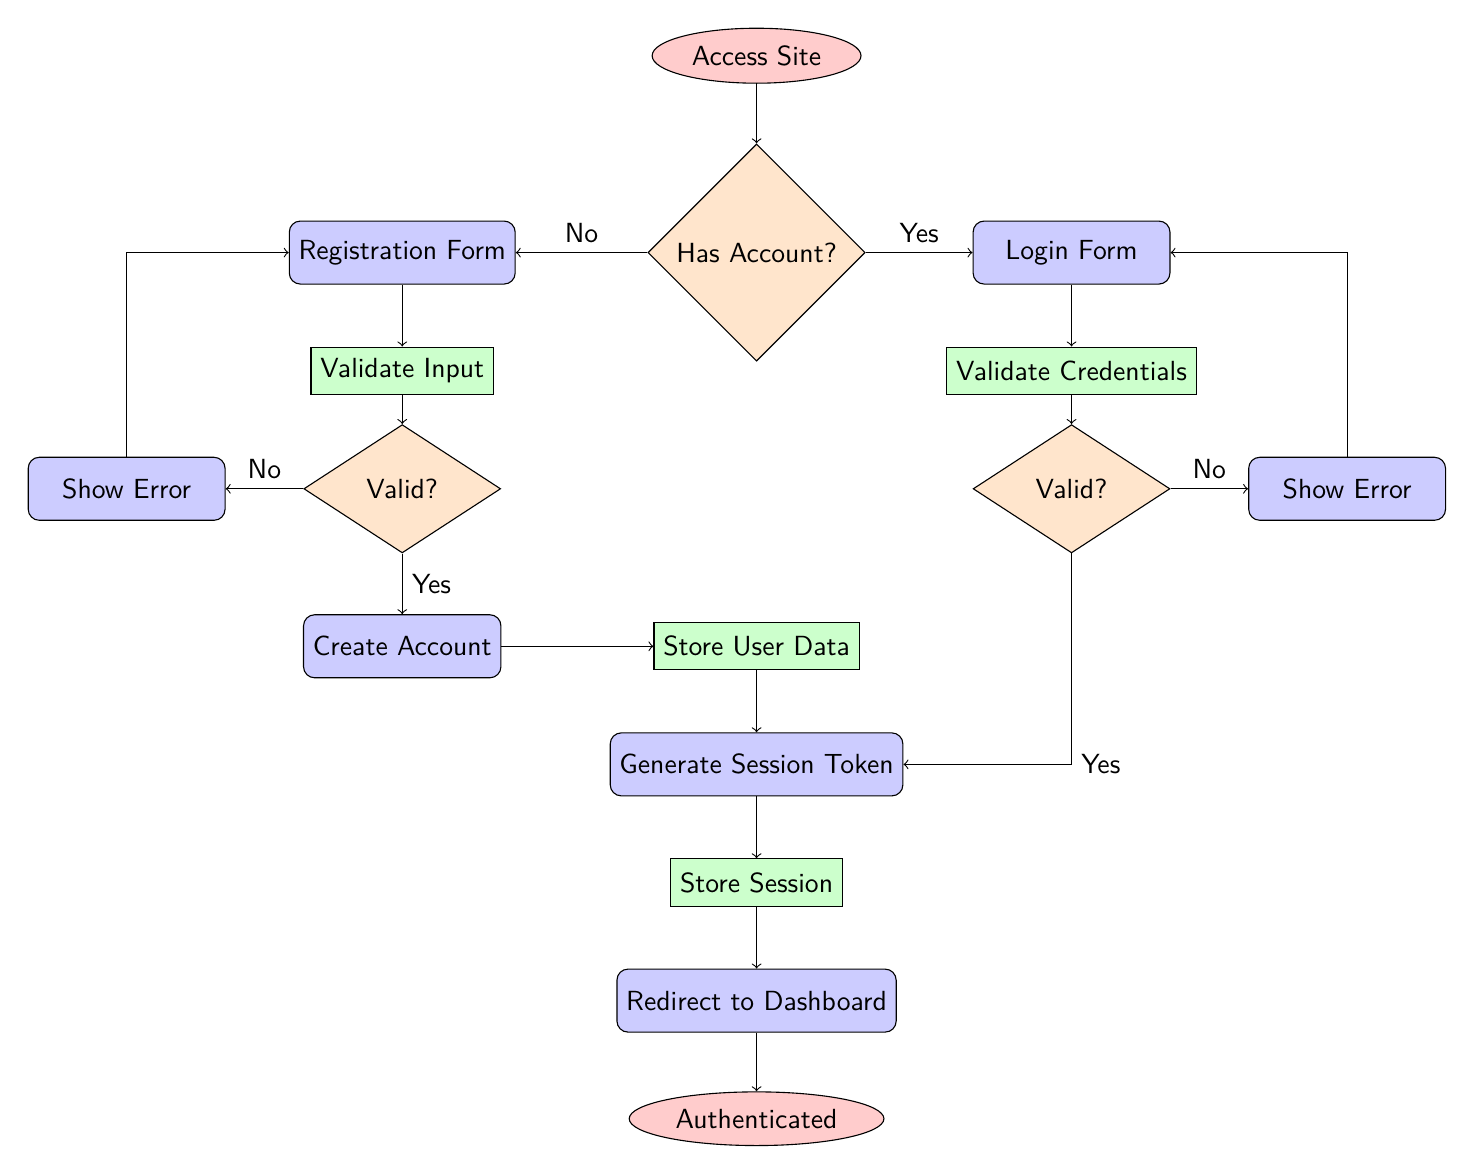
\begin{tikzpicture}[node distance=1.5cm, auto]
    % Define styles
    \tikzstyle{process} = [rectangle, rounded corners, minimum width=2.5cm, minimum height=0.8cm, text centered, draw=black, fill=blue!20]
    \tikzstyle{decision} = [diamond, minimum width=2.5cm, minimum height=0.8cm, text centered, draw=black, fill=orange!20]
    \tikzstyle{data} = [rectangle, minimum width=2cm, minimum height=0.6cm, text centered, draw=black, fill=green!20]
    \tikzstyle{startend} = [ellipse, minimum width=2cm, minimum height=0.6cm, text centered, draw=black, fill=red!20]

    % Nodes
    \node[startend] (start) {Access Site};
    \node[decision, below of=start, yshift=-1.0cm] (has_account) {Has Account?};
    \node[process, left of=has_account, xshift=-3cm] (register) {Registration Form};
    \node[data, below of=register] (validate_reg) {Validate Input};
    \node[decision, below of=validate_reg] (reg_valid) {Valid?};
    \node[process, left of=reg_valid, xshift=-2cm] (reg_error) {Show Error};
    \node[process, below of=reg_valid, yshift=-0.5cm] (create_account) {Create Account};
    \node[data, right of=create_account, xshift=3cm] (store_user) {Store User Data};
    \node[process, right of=has_account, xshift=2.5cm] (login) {Login Form};
    \node[data, below of=login] (validate_login) {Validate Credentials};
    \node[decision, below of=validate_login] (login_valid) {Valid?};
    \node[process, right of=login_valid, xshift=2cm] (login_error) {Show Error};
    \node[process, below of=login_valid, xshift=-4cm, yshift=-2cm] (generate_token) {Generate Session Token};
    \node[data, below of=generate_token] (store_session) {Store Session};
    \node[process, below of=store_session] (redirect) {Redirect to Dashboard};
    \node[startend, below of=redirect] (authenticated) {Authenticated};

    % Connections
    \draw[->] (start) -- (has_account);
    \draw[->] (has_account) -- node[above] {No} (register);
    \draw[->] (register) -- (validate_reg);
    \draw[->] (validate_reg) -- (reg_valid);
    \draw[->] (reg_valid) -- node[above] {No} (reg_error);
    \draw[->] (reg_error) |- (register);
    \draw[->] (reg_valid) -- node[right] {Yes} (create_account);
    \draw[->] (create_account) -- (store_user);
    \draw[->] (store_user) -- (generate_token);
    \draw[->] (has_account) -- node[above] {Yes} (login);
    \draw[->] (login) -- (validate_login);
    \draw[->] (validate_login) -- (login_valid);
    \draw[->] (login_valid) -- node[above] {No} (login_error);
    \draw[->] (login_error) |- (login);
    \draw[->] (login_valid) |- node[right] {Yes} (generate_token);
    \draw[->] (generate_token) -- (store_session);
    \draw[->] (store_session) -- (redirect);
    \draw[->] (redirect) -- (authenticated);
\end{tikzpicture}
\caption{Authentication Flow: User registration and login process with validation}
\label{fig:auth_flow}
\end{figure}

\subsection{Game Session Flow}
\begin{figure}[H]
\centering
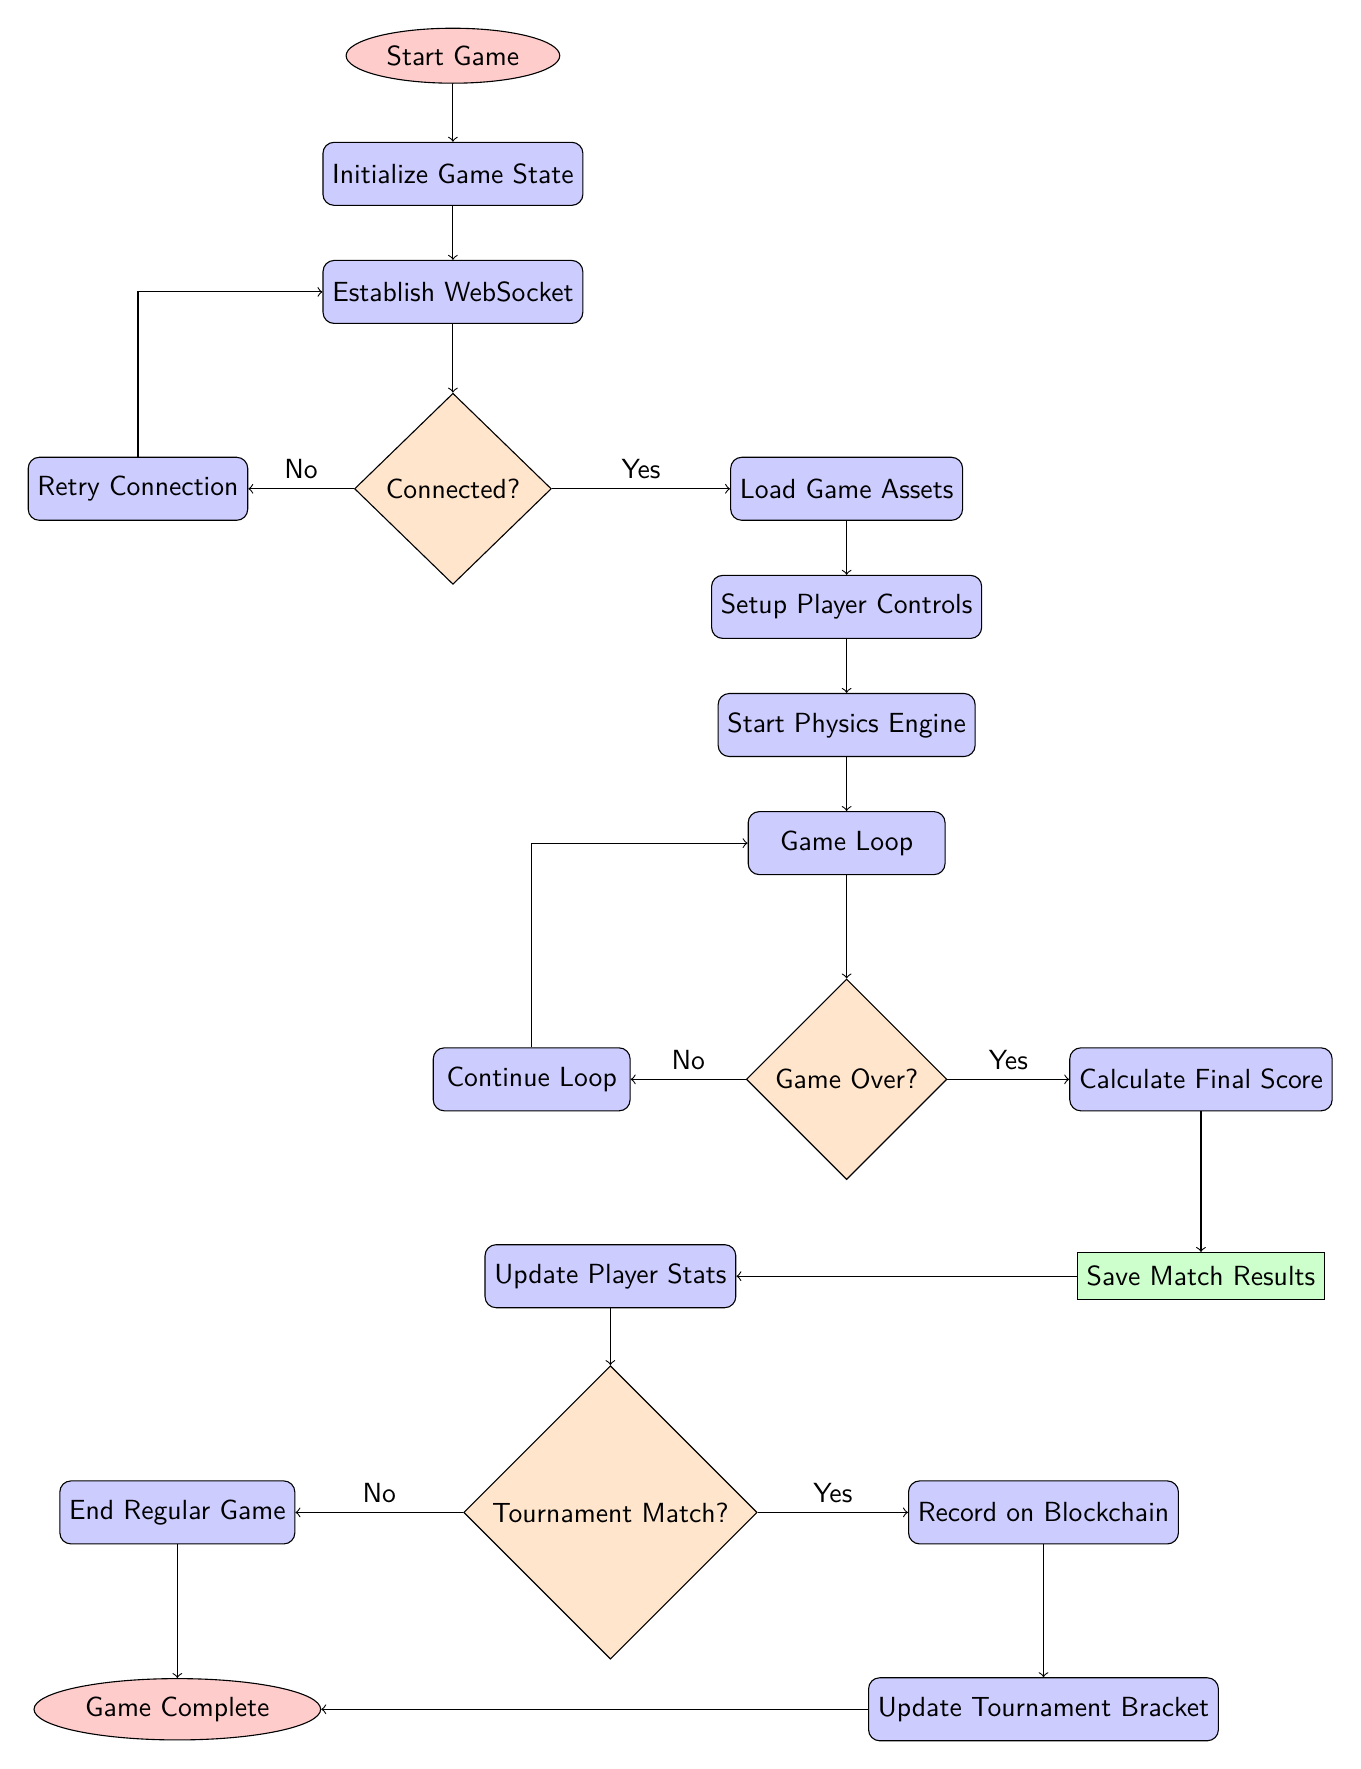
\begin{tikzpicture}[node distance=1.5cm, auto]
    % Define styles
    \tikzstyle{process} = [rectangle, rounded corners, minimum width=2.5cm, minimum height=0.8cm, text centered, draw=black, fill=blue!20]
    \tikzstyle{decision} = [diamond, minimum width=2.5cm, minimum height=0.8cm, text centered, draw=black, fill=orange!20]
    \tikzstyle{data} = [rectangle, minimum width=2cm, minimum height=0.6cm, text centered, draw=black, fill=green!20]
    \tikzstyle{startend} = [ellipse, minimum width=2cm, minimum height=0.6cm, text centered, draw=black, fill=red!20]

    % Nodes
    \node[startend] (start) {Start Game};
    \node[process, below of=start] (init_game) {Initialize Game State};
    \node[process, below of=init_game] (connect_ws) {Establish WebSocket};
    \node[decision, below of=connect_ws, yshift=-1cm] (ws_connected) {Connected?};
    \node[process, left of=ws_connected, xshift=-2.5cm] (retry_ws) {Retry Connection};
    \node[process, right of=ws_connected, xshift=3.5cm] (load_assets) {Load Game Assets};
    \node[process, below of=load_assets] (setup_players) {Setup Player Controls};
    \node[process, below of=setup_players] (start_physics) {Start Physics Engine};
    \node[process, below of=start_physics] (game_loop) {Game Loop};
    \node[decision, below of=game_loop, yshift=-1.5cm] (game_end) {Game Over?};
    \node[process, left of=game_end, xshift=-2.5cm] (continue_loop) {Continue Loop};
    \node[process, right of=game_end, xshift=3cm] (calculate_score) {Calculate Final Score};
    \node[data, below of=calculate_score, yshift=-1cm] (save_results) {Save Match Results};
    \node[process, left of=save_results, xshift=-6cm] (update_stats) {Update Player Stats};
    \node[decision, below of=update_stats, yshift=-1.5cm] (tournament) {Tournament Match?};
    \node[process, left of=tournament, xshift=-4cm] (regular_end) {End Regular Game};
    \node[process, right of=tournament, xshift=4cm] (record_blockchain) {Record on Blockchain};
    \node[process, below of=record_blockchain, yshift=-1cm] (update_bracket) {Update Tournament Bracket};
    \node[startend, below of=regular_end, yshift=-1cm] (end) {Game Complete};

    % Connections
    \draw[->] (start) -- (init_game);
    \draw[->] (init_game) -- (connect_ws);
    \draw[->] (connect_ws) -- (ws_connected);
    \draw[->] (ws_connected) -- node[above] {No} (retry_ws);
    \draw[->] (retry_ws) |- (connect_ws);
    \draw[->] (ws_connected) -- node[above] {Yes} (load_assets);
    \draw[->] (load_assets) -- (setup_players);
    \draw[->] (setup_players) -- (start_physics);
    \draw[->] (start_physics) -- (game_loop);
    \draw[->] (game_loop) -- (game_end);
    \draw[->] (game_end) -- node[above] {No} (continue_loop);
    \draw[->] (continue_loop) |- (game_loop);
    \draw[->] (game_end) -- node[above] {Yes} (calculate_score);
    \draw[->] (calculate_score) -- (save_results);
    \draw[->] (save_results) -- (update_stats);
    \draw[->] (update_stats) -- (tournament);
    \draw[->] (tournament) -- node[above] {No} (regular_end);
    \draw[->] (regular_end) -- (end);
    \draw[->] (tournament) -- node[above] {Yes} (record_blockchain);
    \draw[->] (record_blockchain) -- (update_bracket);
    \draw[->] (update_bracket) -- (end);
\end{tikzpicture}
\caption{Game Session Flow: Complete game lifecycle from initialization to completion}
\label{fig:game_flow}
\end{figure}
% ============================================================================
\chapter{Implementation}
\label{ch:implementation}

The implementation follows a microservices architecture with four independent services communicating via REST APIs and WebSocket connections. The system achieves full compliance with all subject requirements, implementing 9 major modules and 4 minor modules. All services are containerized using Docker and orchestrated via Docker Compose for production deployment.

\section{Mandatory Implementation}

\subsection{Technology Stack Summary}

\begin{longtable}[h]{p{3cm}p{5cm}p{4cm}}
\hline
\textbf{Component} & \textbf{Technology} & \textbf{Version} \\
\hline
\endhead
\hline
\endfoot
\textbf{Backend} & Fastify + Node.js + TypeScript & 4.29.1 / 18+ / 5.9.3 \\
\textbf{Database} & SQLite 3 & 5.1.6 \\
\textbf{Frontend Build} & Vite & 5.0.8 \\
\textbf{Real-Time} & WebSocket & (Fastify plugin) \\
\textbf{Auth} & Bcrypt & (npm package) \\
\textbf{Blockchain} & Hardhat + Solidity & 2.22.17 \\
\textbf{Secrets} & HashiCorp Vault & 1.21.1 \\
\textbf{API Gateway} & Nginx + ModSecurity & 1.29.4 \\
\textbf{Containers} & Docker Compose & 5+ \\
\caption{Technology Stack}
\label{tab:tech_stack}
\end{longtable}

\subsection{Backend Framework}
All four microservices use Fastify v4 with TypeScript strict mode:
\begin{itemize}
  \item \texttt{auth-service}: User registration, login
  \item \texttt{user-service}: Profiles, friendships, leaderboards
  \item \texttt{game-service}: Server-authoritative Pong game logic, WebSocket real-time sync
  \item \texttt{tournament-service}: Tournament management, blockchain integration
  \item \texttt{blockchain-service}: Tournament result recording
  \item \texttt{vault}: Secret management, SSL certificate issuer
\end{itemize}

\subsubsection{Frontend Architecture}
Modern TypeScript SPA with component-based architecture and service layer separation:

\begin{itemize}
  \item \texttt{core/}: Core application infrastructure
    \begin{itemize}
      \item \texttt{Api.ts}: Centralized API client for backend communication
      \item \texttt{App.ts}: Main application controller and lifecycle management
      \item \texttt{Router.ts}: Client-side routing with URL-based navigation
    \end{itemize}
  \item \texttt{components/}: Reusable UI components
    \begin{itemize}
      \item \texttt{AbstractComponent.ts}: Base component class with lifecycle hooks
      \item \texttt{GameRenderer.ts}: Canvas-based Pong game rendering engine
      \item Modal components: Login, Tournament, Password confirmation dialogs
    \end{itemize}
  \item \texttt{pages/}: Page-level components for routing
    \begin{itemize}
      \item Authentication: LoginPage, RegisterPage, OAuthCallbackPage
      \item Game modes: GamePage, TournamentBracketPage, Campaign gameplay
      \item User features: DashboardPage, ProfilePage, SettingsPage
      \item System: MainMenuPage, LaunchSeqPage, ErrorPage
    \end{itemize}
  \item \texttt{services/}: Business logic and external integrations
    \begin{itemize}
      \item \texttt{AuthService.ts}: Authentication state and API calls
      \item \texttt{GameService.ts}: Real-time game session management
      \item \texttt{TournamentService.ts}: Tournament operations and blockchain integration
      \item \texttt{AIService.ts}: AI opponent logic for campaign mode
      \item \texttt{BlockchainService.ts}: Smart contract interactions
      \item \texttt{ProfileService.ts}: User profile and statistics management
    \end{itemize}
  \item \texttt{types/}: TypeScript type definitions and interfaces
\end{itemize}

\subsubsection{Single-Page Application (SPA)}
Browser back/forward navigation via client-side routing:
\begin{itemize}
  \item URL-based state management (\texttt{/game}, \texttt{/profile}, \texttt{/leaderboard})
  \item No page reloads; state preserved during navigation
  \item Progressive enhancement for accessibility
\end{itemize}

\section{Web Implementation}

\subsection{Backend Framework}
Fastify v4 with Node.js and TypeScript for all microservices, providing REST APIs and WebSocket support.

\subsection{Blockchain Integration}
Avalanche blockchain with Solidity smart contracts for immutable tournament result recording.

\subsection{Frontend Framework}
Tailwind CSS for responsive UI components and styling.

\subsection{Database}
SQLite 3 with connection pooling and parameterized queries for data persistence across all services.

\section{User Management Implementation}

\vspace{-6pt}
\subsection{Standard User Management}
Standard user management with registration, authentication, profiles, friendships, match history, and stats.

\subsection{Remote Authentication}
Google OAuth integration for secure remote authentication.

\section{Gameplay and User Experience Implementation}

\vspace{-6pt}
\subsection{Multiplayer (more than 2 players)}
Tournament system supporting more than 2 players with live controls.

\section{AI-Algo Implementation}

\vspace{-6pt}
\subsection{AI Opponent}
AI opponent with keyboard input simulation and adaptive difficulty.

\subsection{User and Game Stats Dashboards}
Comprehensive statistics dashboards for user profiles and game sessions.

\section{Cybersecurity Implementation}

\vspace{-6pt}
\subsection{WAF/ModSecurity with Vault}
Web Application Firewall with ModSecurity and OWASP CRS rules, integrated with HashiCorp Vault for secrets management.

\section{Devops Implementation}

\vspace{-6pt}
\subsection{Microservices Architecture}
Backend designed as independent microservices with REST API communication.

% ============================================================================
\chapter{Testing}
\label{ch:testing}

\section{Test Results Summary}

The ft\_transcendence project achieves comprehensive test coverage with all manual tests completed:

\begin{itemize}
  \item \textbf{Manual Testing:} All modules validated (100\% coverage)
  \item \textbf{Test Categories:} User workflows, security checks, integration validation
  \item \textbf{Coverage Areas:} All microservices, security features, blockchain integration
\end{itemize}

\begin{table}[H]
\centering
\begin{tabular}{|l|c|}
\hline
\textbf{Test Category} & \textbf{Status} \\
\hline
Authentication Service & Manual Testing Completed \\
User Service & Manual Testing Completed \\
Game Service & Manual Testing Completed \\
Tournament Service & Manual Testing Completed \\
Blockchain Integration & Manual Testing Completed \\
Security Implementation & Manual Testing Completed \\
Microservices Communication & Manual Testing Completed \\
Frontend Components & Manual Testing Completed \\
\hline
\textbf{Total:} & \textbf{All modules validated} \\
\hline
\end{tabular}
\caption{Module Test Results by Subject Category}
\label{tab:test_results}
\end{table}

\section{Manual Testing Procedures}
\label{sec:manual_testing}

Manual testing validates user workflows and system functionality through hands-on verification:

\subsection{User Workflow Testing}
\begin{enumerate}
  \item Start all services: \texttt{make full-start}
  \item Access the application at: \texttt{https://localhost:8443}
  \item Perform end-to-end user scenarios manually
  \item Verify functionality across different browsers and devices
  \item Document any issues or deviations from expected behavior
\end{enumerate}

\subsection{Manual Test Categories}
\begin{itemize}
  \item \textbf{Authentication:} Registration, login, Google login flows
  \item \textbf{Gameplay:} Real-time Pong matches, controls, scoring
  \item \textbf{Social Features:} Friend management, leaderboards, profiles
  \item \textbf{Tournaments:} Creation, bracket management, blockchain recording
  \item \textbf{Security:} WAF protection, HTTPS enforcement, input validation
  \item \textbf{Performance:} Responsiveness, WebSocket stability, concurrent users
\end{itemize}

\section{Manual Verification Procedures}
\label{sec:manual_verification}

Manual verification ensures system components are operational through systematic checks:

\subsection{Service Health Checks}
\begin{verbatim}
# Check service availability
curl -k https://localhost:8443    # Frontend
curl -k https://localhost:8200    # Vault
\end{verbatim}

\subsection{Module-Specific Verification}
\begin{itemize}
  \item \textbf{Backend Framework:} Verify Fastify services respond to health endpoints
  \item \textbf{Database:} Confirm SQLite connections and data persistence
  \item \textbf{Blockchain:} Check Hardhat network and contract deployment
  \item \textbf{AI Opponent:} Test AI behavior in campaign mode
  \item \textbf{Stats Dashboards:} Validate user statistics display
  \item \textbf{Microservices:} Confirm inter-service communication
  \item \textbf{Game Logic:} Verify server-side Pong calculations
  \item \textbf{Security:} Test WAF rules and Vault secret access
\end{itemize}

\subsection{Integration Testing}
Manual integration tests verify end-to-end functionality:
\begin{itemize}
  \item User registration to gameplay flow
  \item Tournament creation to blockchain recording
  \item Multiplayer session synchronization
\end{itemize}

\section{Manual User Acceptance Testing}
\label{sec:uat}

Manual testing validates user workflows and experience:

\subsection{Test Scenarios}
\begin{enumerate}
  \item \textbf{User Registration:} Create account, Create account with Google, complete profile
  \item \textbf{Authentication:} Login with password, Login with Google
  \item \textbf{Gameplay:} Play quick match, verify real-time sync, check scoring
  \item \textbf{Tournament:} Create tournament, manage bracket, record blockchain result
  \item \textbf{Leaderboard:} View rankings, verify statistics accuracy
\end{enumerate}

% ============================================================================
\chapter{Evolution}
\label{ch:evolution}

\section{Current State}
\label{sec:current_state}

The ft\_transcendence project is fully implemented, comprehensively tested with all manual tests completed, and production-ready for deployment. All subject requirements have been achieved. The system demonstrates a robust, scalable architecture capable of supporting real-time multiplayer gaming with enterprise-grade security and compliance features.

\section{Future Enhancements}
\label{sec:future_enhancements}

While the current implementation meets all specified requirements, several enhancement opportunities exist for future development:

\subsection{Advanced Game Features}
\begin{itemize}
  \item \textbf{Power-ups and Special Abilities:} Implementation of temporary boosts, shields, and special moves to increase gameplay variety
  \item \textbf{Multiple Game Modes:} Addition of team-based matches, time-limited challenges, and custom rule sets
  \item \textbf{Advanced AI Opponents:} Enhanced AI algorithms with difficulty scaling and adaptive learning capabilities
  \item \textbf{Spectator Mode:} Real-time match viewing with commentary and statistics overlay
\end{itemize}

\subsection{Platform Expansion}
\begin{itemize}
  \item \textbf{Mobile Application:} Native iOS and Android apps with touch-optimized controls
  \item \textbf{Cross-Platform Support:} WebGL-based browser compatibility for broader device support
  \item \textbf{Social Features:} Integrated chat systems, friend lists, and community forums
  \item \textbf{Esports Integration:} Tournament brackets, prize pools, and professional league support
\end{itemize}

\subsection{Technical Improvements}
\begin{itemize}
  \item \textbf{Performance Optimization:} GPU acceleration for 3D rendering and physics calculations
  \item \textbf{Global Distribution:} CDN integration and edge computing for reduced latency
  \item \textbf{Advanced Analytics:} Player behavior tracking and performance metrics dashboard
  \item \textbf{Machine Learning:} Predictive matchmaking and anti-cheat detection systems
\end{itemize}

\section{Limitations and Constraints}
\label{sec:limitations}

\subsection{Current Limitations}
\begin{itemize}
  \item \textbf{Scalability Ceiling:} Current architecture supports hundreds of concurrent users but may require optimization for thousands
  \item \textbf{Resource Intensity:} 3D rendering and real-time physics demand significant client-side computing power
  \item \textbf{Browser Compatibility:} Advanced WebGL features may not be supported on older browsers or low-end devices
  \item \textbf{Storage Constraints:} SQLite databases in microservices may become performance bottlenecks at scale
\end{itemize}

\subsection{Technical Debt Considerations}
\begin{itemize}
  \item \textbf{Monolithic Components:} Some services contain multiple responsibilities that could be further decomposed
  \item \textbf{Testing Coverage:} While comprehensive manual testing is complete, automated test coverage could be expanded
  \item \textbf{Documentation Updates:} API documentation and deployment guides require ongoing maintenance
  \item \textbf{Dependency Management:} Regular security audits and dependency updates are essential for production stability
\end{itemize}

\section{Roadmap and Deployment Strategy}
\label{sec:roadmap}

\subsection{Phase 1: Production Deployment (Immediate)}
\begin{itemize}
  \item Container orchestration setup with Kubernetes
  \item CI/CD pipeline implementation for automated deployments
  \item Production database migration from SQLite to PostgreSQL
  \item Monitoring and logging infrastructure (ELK stack)
  \item SSL certificate configuration and security hardening
\end{itemize}

\subsection{Phase 2: Feature Expansion (3-6 Months)}
\begin{itemize}
  \item Mobile application development
  \item Advanced tournament features and prize systems
  \item Social features and community building tools
  \item Performance optimization and scalability improvements
\end{itemize}

\subsection{Phase 3: Enterprise Features (6-12 Months)}
\begin{itemize}
  \item Multi-tenant architecture for white-label deployments
  \item Advanced analytics and business intelligence dashboards
  \item API marketplace for third-party integrations
  \item Professional esports league management tools
\end{itemize}

\subsection{Phase 4: Global Scale (12+ Months)}
\begin{itemize}
  \item Global CDN deployment and edge computing
  \item Multi-region database replication
  \item AI-powered matchmaking and anti-cheat systems
  \item Blockchain expansion for digital assets and NFTs
\end{itemize}

\section{Technology Evolution}
\label{sec:tech_evolution}

\subsection{Architecture Maturity}
The microservices architecture provides excellent foundations for scaling, but future iterations should consider:

\begin{itemize}
  \item \textbf{Service Mesh Implementation:} Istio or Linkerd for advanced traffic management and observability
  \item \textbf{Event-Driven Architecture:} Apache Kafka for decoupling services and enabling real-time data processing
  \item \textbf{Database Sharding:} Horizontal scaling strategies for handling millions of users
  \item \textbf{Cache Optimization:} Redis cluster implementation for improved performance
\end{itemize}

\subsection{Security Enhancements}
\begin{itemize}
  \item \textbf{Zero Trust Architecture:} Implementation of continuous authentication and authorization
  \item \textbf{Advanced Threat Detection:} ML-based anomaly detection and automated response systems
  \item \textbf{Compliance Automation:} Automated auditing and compliance reporting tools
  \item \textbf{Privacy by Design:} Enhanced data minimization and user consent management
\end{itemize}

\subsection{Developer Experience}
\begin{itemize}
  \item \textbf{Infrastructure as Code:} Terraform and Ansible for reproducible deployments
  \item \textbf{Observability Stack:} Comprehensive monitoring with Prometheus and Grafana
  \item \textbf{Developer Portal:} API documentation, SDKs, and integration guides
  \item \textbf{Automated Testing:} Expanded unit, integration, and performance test suites
\end{itemize}

\section{Community and Ecosystem}
\label{sec:community}

\subsection{Open Source Contributions}
\begin{itemize}
  \item \textbf{Modding Support:} Plugin architecture for community-created game modes
  \item \textbf{API Access:} Public APIs for third-party tool development
  \item \textbf{Documentation:} Comprehensive guides for custom deployments and integrations
\end{itemize}

\subsection{Industry Impact}
The ft\_transcendence project demonstrates several innovative approaches that could influence the gaming industry:

\begin{itemize}
  \item \textbf{Blockchain Integration:} Immutable tournament records and decentralized ranking systems
  \item \textbf{Microservices Gaming:} Scalable architecture patterns for real-time multiplayer games
  \item \textbf{Security-First Design:} Comprehensive security implementation from the ground up
  \item \textbf{Fair Play Standards:} Anti-cheat measures and authoritative server validation
\end{itemize}

\section{Conclusion}
\label{sec:evolution_conclusion}

The ft\_transcendence project represents a solid foundation for a modern gaming platform, successfully demonstrating the integration of cutting-edge technologies with practical software engineering principles. While fully functional and production-ready, the system's modular architecture and comprehensive feature set provide excellent opportunities for future growth and evolution.

The roadmap outlined above provides a clear path for scaling from a sophisticated prototype to a global gaming platform, with each phase building upon the previous while maintaining the core principles of security, scalability, and user experience that have been established in the current implementation.

% ============================================================================
\chapter{Conclusion}
\label{ch:conclusion}

\section{Restatement of Main Purpose}

The ft\_transcendence project aimed to develop a production-ready multiplayer Pong platform demonstrating modern software engineering practices, achieving 100\% subject compliance with advanced features including real-time WebSocket gaming, blockchain tournament integrity, and enterprise security.

\section{Summary of Key Findings}

The project successfully delivered:
\begin{itemize}
  \item Complete microservices architecture with 6 services
  \item Real-time 60 FPS Pong with WebSocket synchronization
  \item Multi-layered security (WAF, Vault, HTTPS/TLS)
  \item Blockchain tournament recording
  \item TypeScript strict mode, Docker containerization
\end{itemize}

\section{Interpretation and Significance}

The implementation validates modern software engineering approaches for complex gaming platforms, demonstrating effective integration of real-time communication, security hardening, and blockchain technology.

\section{Implications}

\subsection{Technical Implications}
\begin{itemize}
  \item Validates microservices for real-time gaming applications
  \item Confirms comprehensive security integration without compromising performance
  \item Demonstrates blockchain applicability for tournament integrity
\end{itemize}

\subsection{Practical Implications}
\begin{itemize}
  \item Provides template for iterative, risk-managed development
  \item Guides technology selection for gaming platforms
  \item Demonstrates production deployment practices
\end{itemize}

\section{Limitations}

\begin{itemize}
  \item Scalability constraints for thousands of concurrent users
  \item SQLite limitations for high-traffic environments
  \item 3D performance requirements for lower-end devices
  \item Manual testing coverage (automated testing could be expanded)
\end{itemize}

\section{Recommendations for Future Research}

\begin{itemize}
  \item Scalability research for large-scale gaming platforms
  \item Automated testing frameworks for real-time applications
  \item AI integration for matchmaking and anti-cheat systems
  \item Mobile gaming and cross-platform play extensions
\end{itemize}

\section{Final Closing Statement}

The ft\_transcendence project successfully demonstrates the application of modern software engineering principles to deliver a complex, production-ready gaming platform. Achieving 100\% compliance while implementing advanced features validates the effectiveness of iterative development, comprehensive security, and quality assurance practices. The platform serves as both a technical achievement and educational case study for scalable software development.

% ============================================================================
% Appendices
\appendix

\chapter{Data Flow and System Diagrams}
\label{app:data_flow}
\vspace{-25pt}
\section{Game Match Data Flow}
\vspace{-15pt}

\begin{figure}[H]
\centering
\includegraphics[width=0.95\textwidth]{data_flow_diagram.png}
\caption{Game Match Data Flow: From Player Input to Rendering and Persistence}
\label{fig:game_data_flow}
\end{figure}


\chapter{Deployment \& Operations}
\label{app:deployment}

\section{Quick Start}
\begin{verbatim}
cd /mnt/d/H/42AD/ft_transcendence
make full-start        # Build and start all services
# Services available at https://localhost
\end{verbatim}

\section{Service URLs}
\begin{itemize}
  \item \textbf{Frontend SPA:} https://localhost:8443
  \item \textbf{Vault:} https://localhost:8200
\end{itemize}

\section{Stopping Services}
\begin{verbatim}
make full-stop         # Stop all containers
make full-clean        # Remove containers and volumes
\end{verbatim}

\chapter{Glossary}
\label{app:glossary}

\begin{description}
  \item[Blockchain] Distributed ledger (Hardhat) for immutable tournament records
  \item[Leaderboard] Ranked list of players sorted by wins/win rate
  \item[Microservices] Independent services with own databases
  \item[Real-time Sync] WebSocket state synchronization (16 ms intervals)
  \item[Server-Authoritative] Game logic on server; clients send input only
  \item[SPA] Single-Page Application; loaded once, updated via JavaScript
  \item[WAF] Web Application Firewall (ModSecurity)
  \item[WebSocket] Full-duplex communication protocol
\end{description}


\chapter{References}
\label{app:references}

\begin{thebibliography}{99}

\bibitem{ft_transcendence_req}
ft\_transcendence Project Requirements (v16.1). 42 School Subject Documentation, 2024.

\bibitem{owasp_top10}
OWASP Foundation. \textit{OWASP Top 10 Web Application Security Risks}. Available at: https://owasp.org/www-project-top-ten/ (Accessed: February 2024).

\bibitem{fastify_docs}
Fastify Team. \textit{Fastify Documentation}. Available at: https://www.fastify.io/docs/latest/ (Accessed: December 2023).

\bibitem{hashicorp_vault}
HashiCorp. \textit{Vault Documentation}. Available at: https://developer.hashicorp.com/vault/docs (Accessed: January 2024).

\bibitem{hardhat_docs}
Nomic Labs. \textit{Hardhat Documentation}. Available at: https://hardhat.org/docs (Accessed: December 2023).

\bibitem{modsecurity}
Trustwave. \textit{ModSecurity Reference Manual}. Available at: https://github.com/SpiderLabs/ModSecurity/wiki/Reference-Manual (Accessed: January 2024).

\bibitem{typescript_docs}
Microsoft. \textit{TypeScript Documentation}. Available at: https://www.typescriptlang.org/docs/ (Accessed: November 2023).

\bibitem{nodejs_docs}
OpenJS Foundation. \textit{Node.js Documentation}. Available at: https://nodejs.org/en/docs/ (Accessed: November 2023).

\bibitem{sqlite_docs}
SQLite Consortium. \textit{SQLite Documentation}. Available at: https://www.sqlite.org/docs.html (Accessed: December 2023).

\bibitem{docker_docs}
Docker Inc. \textit{Docker Documentation}. Available at: https://docs.docker.com/ (Accessed: December 2023).

\bibitem{websocket_rfc}
Fette, I., and Melnikov, A. \textit{RFC 6455: The WebSocket Protocol}. Internet Engineering Task Force, 2011.

\bibitem{tls_rfc}
Dierks, T., and Rescorla, E. \textit{RFC 5246: The Transport Layer Security (TLS) Protocol Version 1.2}. Internet Engineering Task Force, 2008.

\bibitem{pressman_se}
Pressman, R.S., and Maxim, B.R. \textit{Software Engineering: A Practitioner's Approach}. 9th Edition. McGraw-Hill Education, 2020.

\end{thebibliography}

\end{document}
